%\documentclass{class-for-drafts}
\documentclass[english,a4paper]{lipics-v2018}
\nolinenumbers

%% url
\usepackage{hyperref, url}
%% maths
\usepackage{amsmath,amssymb,bm}
%% algorithms
\usepackage{algorithmicx}
\usepackage[ruled, linesnumbered, noend]{algorithm2e}
\usepackage{multicol}

\usepackage{pifont}

%% images
\usepackage{graphicx}
%\usepackage[dvipsnames]{xcolor}
%% inparaenum
\usepackage{paralist}
\usepackage{enumitem}
%% tables
\usepackage{booktabs,multirow,tabularx,hhline}
\usepackage{makecell}
%% figures
%\usepackage{caption}
% \usepackage{subfig}
%\usepackage[font=small, skip=2pt]{caption}
%\usepackage[font=small]{subfig}
\usepackage{tikz}
\usetikzlibrary{arrows.meta,decorations.pathreplacing,decorations.pathmorphing,plotmarks,shapes,matrix,patterns}
\usepackage[normalem]{ulem}
\tikzset{>={Latex[width=3pt,length=5pt]}}
%% transform eps in pdf crossplateform
\usepackage{epsfig}
\usepackage{epstopdf}

%% hyphenation
\usepackage{hyphenat}
\hyphenation{brow-sers brow-ser}

\newcommand{\TODO}[1]{\textcolor{red}{#1}}
\newcommand{\REF}[0]{\textcolor{purple}{REF}}
\newcommand{\COLOR}[2]{\textcolor{#1}{#2}}

\usepackage{xspace}
\newcommand{\SCAMP}[0]{\textsc{Scamp}\xspace}
\newcommand{\CYCLON}[0]{\textsc{Cyclon}\xspace}
\newcommand{\SPRAY}[0]{\textsc{Spray}\xspace}
\newcommand{\LSEQ}[0]{\textsc{LSeq}\xspace}
\newcommand{\CRATE}[0]{\textsc{Crate}\xspace}
\newcommand{\PEERSIM}[0]{\textsc{PeerSim}\xspace}

\newcommand{\PCBROADCAST}[0]{\textup{PC-broadcast}\xspace}
\newcommand{\RPCBROADCAST}[0]{\textup{PRC-broadcast}\xspace}

\usepackage{amsthm} %% proof env
% \newtheorem{definition}{Definition}
% \newtheorem{theorem}{Theorem}
% \newtheorem{lemma}{Lemma}
\newtheorem*{problem*}{Problem statement}

\newcommand{\EXAMPLE}[2]{\noindent \textbf{\emph{#1}} #2}
\newcommand{\PAR}[2]{\noindent \textbf{#1} #2}

%%%%%%%%%%%%%%%%%%%%%%%%%%%%%%%%%%%%%%%%%%%%%%%%%%%%%%%%%%%%%%%%%%%%%%%%%%%%%%%
%%%%%%%%%%%%%%%%%%%%%%%%%%%%%%%%%%%%%%%%%%%%%%%%%%%%%%%%%%%%%%%%%%%%%%%%%%%%%%%
%%%%%%%%%%%%%%%%%%%%%%%%%%%%%%%%%%%%%%%%%%%%%%%%%%%%%%%%%%%%%%%%%%%%%%%%%%%%%%%

\newcommand{\affLSNN}{LS2N, University of Nantes,
   2 rue de la Houssini{\`e}re,
   BP 92208, 44322 Nantes Cedex 3, France}%,
%   \url{first.last@univ-nantes.fr}}

 \author{Brice N{\'e}delec}{\affLSNN}{brice.nedelec@ls2n.fr}{}{}
 \author{Pascal Molli}{\affLSNN}{pascal.molli@ls2n.fr}{}{}
 \author{Achour Most{\'e}faoui}{\affLSNN}{achour.mostefaoui@ls2n.fr}{}{}

\authorrunning{B. N{\'e}delec, P. Molli and A. Most{\'e}faoui}

\keywords{Causal broadcast, complexity trade-off, large and dynamic systems}

\Copyright{Brice N{\'e}delec, Pascal Molli and Achour Most{\'e}faoui}

\subjclass{\ccsdesc[300]{Computer systems organization~Peer-to-peer architectures}}


\EventEditors{Jiannong Cao, Faith Ellen, Luis Rodrigues, and Bernardo Ferreira}
\EventNoEds{4}
\EventLongTitle{22nd International Conference on Principles of Distributed Systems (OPODIS 2018)}
\EventShortTitle{OPODIS 2018}
\EventAcronym{OPODIS}
\EventYear{2018}
\EventDate{December 17–19, 2018}
\EventLocation{Hong Kong, China}
\EventLogo{}
\SeriesVolume{122}
\ArticleNo{0}


\section*{Acknowledgments}

This work was % partially
funded by
% the French ANR project SocioPlug
% (ANR-13-INFR-0003), and by
the DeSceNt project granted by the Labex CominLabs excellence laboratory
(ANR-10-LABX-07-01).

% Experiments presented in this paper were carried out using the Grid'5000
% testbed, supported by a scientific interest group hosted by Inria and including
% CNRS, RENATER and several Universities as well as other organizations (see
% \url{https://www.grid5000.fr}).

% \lipsum[56]

%%% Local Variables:
%%% mode: latex
%%% TeX-master: "../paper"
%%% End:


\begin{document} 

\title{Causal Broadcast: How to Forget?}

\maketitle


%\IEEEtitleabstractindextext{
\begin{abstract}
  Causal broadcast constitutes the fundamental communication primitive of many
  distributed protocols and applications. However, state-of-the-art
  implementations fail to forget obsolete control information about past
  delivered messages. They do not scale in large and dynamic systems.  In this
  paper, we propose a novel implementation of causal broadcast.  We prove that
  all and only obsolete control information is safely removed, at cost of a few
  lightweight control messages. Local space complexity is not monotonically
  increasing and depends on system settings and use.  Message overhead is
  constant.  Our implementation constitutes a sustainable communication
  primitive for causal broadcast in large and dynamic systems.
\end{abstract}
%}

% \begin{abstract}
%   Causal broadcast constitutes the core communication primitive of many
%   distributed systems. For decades, state-of-the-art approaches relied on
%   maintaining and transmitting vector clocks. The size of vector clocks
%   increases linearly with the number of processes that ever entered the
%   system. Causal broadcast eventually became overcostly and inefficient in large
%   and dynamic systems.  A recent approach solved the issue about generated
%   traffic by removing the need for transmitting vectors. However, it still
%   maintains a vector locally. In this paper, we improve this causal broadcast by
%   removing the need for such vector. The proposed protocol safely purges the
%   local structure over time at cost of few control messages. As consequence,
%   causal broadcast can run in large and dynamic systems even on most humble
%   devices such as Raspberry Pi's.
% \end{abstract}

% \keywords{Causal broadcast, local space complexity}


%%% Local Variables:
%%% mode: latex
%%% TeX-master: "../paper"
%%% End:


 
\section{Introduction}

Causal broadcast (\REF) constitutes the core communication primitive of many
distributed systems (\REF). It ensures the reliable delivery of broadcast
messages, exactly once, following Lamport's happen before
relationship~\cite{lamport1978time}. If the sending of a message $m$ precedes
the sending of a message $m'$ then all processes that deliver these two messages
need to deliver $m$ before $m'$. Otherwise they deliver them in any order.

In large and dynamic systems, processes cannot afford to maintain an up-to-date
knowledge of the full membership. Instead, each process builds a partial view of
neighbors to communicate with. Gossiping exploits these neighborhoods to
efficiently broadcast a message to all processes. To broadcast a message, a
process sends the message to its neighbors; each process receiving such message
forwards it to its own neighbors. Processes receive the message either directly
or transitively. Processes may receive a broadcast message multiples times from
different sources.  To deliver each message exactly once, reliable broadcast
must discard the additional copies of the original message at receipt. 

In static systems where processes cannot join, leave, or self-reconfigure their
neighborhood, the local structure that ensures exactly once delivery is
lightweight.  Since each process forwards each message exactly once, each
process knows that it will receive a number of copies of the original message
equal to the number of their incoming links. Once it received that many copies,
it safely purges its local structure from this message. It will never receive
this message again.

This does not hold in dynamic systems. When a process adds a neighbor to its
partial view, the latter does not know if it should expect another message copy 
from this new incoming link. \TODO{Need to be more accurate.}  To solve this,
causal broadcast relies on reliable broadcast which takes a vector the size of
which is linear with the number of processes that ever broadcast a message
(\REF).

% State-of-the-art causal broadcasts (\REF) reuse this vector of clocks. Each
% message piggybacks such vector to ensure their causal delivery. A recent causal
% broadcast (\REF) alleviates processes from the need for piggybacking vectors in
% messages. However, it still requires to maintain the local vector to ensure that
% it delivers each message exactly once.

In this paper, we present a causal broadcast protocol that extends (\REF).  Our
contribution is twofold:
\begin{itemize}
\item We describe a causal broadcast that piggybacks constant size control
  information while maintaining a local structure that is safely purged over
  time, and we prove it.
\item We provide experiments that highlight \TODO{something}.
\end{itemize}
While (\REF) solves the issue about generated traffic, our approach solves the
issue about local space consumption. As consequence, causal broadcast can run in
large and dynamic systems even on most humble devices such as Raspberry Pi’s.



The rest of this paper is organized as follows. Section~\ref{sec:motivations}
shows the issue and motivates this work. Section~\ref{sec:proposal} presents the
proposed causal broadcast and corresponding
proofs. Section~\ref{sec:experimentation} highlights the pros and cons of our
approach on experimental setups. We conclude in Section~\ref{sec:conclusion}.


%%% Local Variables:
%%% mode: latex
%%% TeX-master: "../paper"
%%% End:


\section{Proposal}
\label{sec:proposal}

In this section, we present a causal broadcast protocol providing an original
tradeoff in terms of complexity. It removes the last linear and monotonic upper
bound that remained on space complexity at the cost of few lightweight control
messages. The key ideas are:
\begin{enumerate}
\item Each process broadcasts or forwards a message once, hence each link convey
  a message once. After the first receipt, the process expects to receive
  another copy of this message from each other link pointing to it. Once the
  process received all copies, the control information associated to the message
  is entirely and safely removed.
\item Adding links between processes adds uncertainty. Processes cannot tell if
  they should expect a message from a link any longer.
\item By exploiting causal order, processes remove this uncertainty. Causal
  order allows to remove batches of obsolete information while reasoning about
  temporarily buffered broadcast messages. In this paper, we exploit causal
  broadcast to improve its underlying reliable broadcast.
\end{enumerate}

\subsection{Model}

A distributed system comprises a set of processes that can communicate with each
other using messages. Processes may not have full knowledge of the membership of
the system. Instead, processes build and maintain overlay networks: each process
updates a local partial view of logical communication links, i.e., a set of
processes to communicate with. The partial view is usually much smaller than the
actual system size. We speak of overlay networks, networks, or distributed
systems indifferently.

\begin{definition}[Overlay network]
  An overlay network $G: P \times E$ comprises a set of processes $P$ and a set
  of directed links $E: P \times P$.  An overlay network is static if both sets
  $P$ and $G$ are immutable. Otherwise, the overlay network is dynamic. An
  overlay network is unpartitioned if their exists a path -- i.e. a link or an
  array of links -- from any process to any other process. We only consider
  unpartitioned overlay networks.
\end{definition}

\begin{definition}[Process]
  A process runs a set of instructions sequentially. Processes communicate with
  each other using asynchronous message passing. A process~A can send a message
  to another process~B $s_{AB}(m)$, or to any process $s_A(m)$; receive a
  message from another process~B $r_{AB}(m)$, or from any process $r_A(m)$. A
  process sends messages to the set of links departing from it, called
  neighborhood, or partial view, or out-view $Q_o$. A process receives messages
  from the set of links arriving to it, called in-view $Q_i$.  Processes are
  faulty if they crash, otherwise they are correct. We do not consider byzantine
  processes.
\end{definition}

Causal broadcast relies on reliable broadcast that provides guarantees on
message delivery. Each process receives each broadcast message at least once and
delivers it once despite possible multiple receipts.

\begin{definition}[\label{def:reliablebroadcast}Uniform reliable broadcast] 
  When a process~A broadcasts a message to all processes of its system $b_A(m)$,
  each correct process~B eventually receives it and delivers it
  $d_B(m)$. Uniform reliable broadcast guarantees 3 properties:
  \begin{itemize}[leftmargin=*]
  \item Validity: If a correct process broadcasts a message, then it
    eventually delivers it.
  \item Uniform Agreement: If a process -- correct or not -- delivers a message,
    then all correct processes eventually deliver it.
  \item Uniform Integrity: A process delivers a message at most once, and only if
    it was previously broadcast.
  \end{itemize}
\end{definition}

Definition~\ref{def:reliablebroadcast} suggests the use of data structures that
saves delivered messages to ignore additional receipts. In static systems, such
data structure can be non-monotonic~\cite{raynal2013distributed}. We define a
non-monotonic link-wise memory to forbid multiple delivery.

\begin{definition}[\label{def:memory}Link memory]
  A link from Process~A to Process~B remembers among Process~B's delivered
  messages those that will be received from Process~A; and forgets among
  Process~B's delivered messages those that will never be received from
  Process~A.\\
  $\forall m,\, remember_{BA}(m) \equiv d_B(m) \wedge \neg r_{BA}(m)$ \\
  $\forall m,\, remember_{BA}(m) \implies r_{BA}(m)$
\end{definition}


\begin{theorem}[Link memory forbids multiple delivery]
  Assuming that each link conveys each message at most once, link memory is
  sufficient to forbid multiple delivery.
\end{theorem}

\begin{proof}
  We must show that
  $\not\exists m, d_B(m) \rightarrow r_{BA}(m) \wedge r_{BA}(m) \rightarrow
  d_B(m)$.
  The delivery $d_B(m)$ implies a prior receipt $r_B(m)$.  To deliver $m$ after
  its receipt from Process~A, Process~B must not remember $m$ on this link.  If
  Process~B does not remember $m$ from Process~A, either it already received $m$
  from Process~A; or it did not received $m$ from any process. In the former
  case, it cannot receive, hence deliver, $m$ from Process~A; in the latter
  case, receiving $m$ from Process~A leads to the delivery of $m$. Again, since
  a link conveys a message at most once, it cannot receive another $m$ from
  Process~A that would lead to another delivery.
\end{proof}


\begin{algorithm}[h]
  \SetKwProg{Function}{function}{}{}
\SetKwProg{Upon}{upon}{}{}
\SetKwProg{Initially}{INITIALLY:}{}{}
\SetKwProg{Dissemination}{DISSEMINATION:}{}{}

\small

\DontPrintSemicolon
\LinesNumbered

%\Initially {} {
  $Q_o$ \tcp*{Out-view}
  $Q_i$ \tcp*{In-view}
  \BlankLine
  $E \leftarrow \varnothing$ \tcp*{\footnotesize Map of expected messages $Q_i : M^*$}
%}

\BlankLine

\Dissemination{}{

  \begin{multicols}{2}

  \Function{$\textup{C-broadcast}(m)$} { %\tcp*[f]{$b_p(m)$}} { 
    % $\textup{received}(m,\, \_)$ \;
    % \lForEach {$q \in Q_o$} {\textup{sendTo}($q,\, m$)}
    % \textup{R-deliver}($m$) \; % \tcp*{$d_p(m)$}
    $\textup{receive}(m,\, \_)$ \;
  }

  \BlankLine
  
  \Upon{$\textup{receive}(m,\, l)$}{
    \If {$\neg\textup{received}(m,\,l)$} {
      \lForEach {$q \in Q_o$} {\textup{sendTo}($q,\, m$)}
      % \tcp*[f]{broadcast or forward}}
      \textup{C-deliver}($m$) \; % \tcp*{$d_p(m)$}
    }
  }

  \BlankLine
  
  \Function{$\textup{received}(m,\, l)$}{
    $rcvd \leftarrow
    \exists q \in E$ \textbf{\textup{with}} $m\in E[q]$ \;
    \If {$\neg rcvd$} {
      \ForEach {$q \in Q_i$} {$E[q] \leftarrow E[q] \cup m$ \label{line:remembers}}
        % \tcp*[f]{to remember}}
    }
    $E[l] \leftarrow E[l] \setminus m$ \label{line:forgets} \;%\tcp*{to forget}
    \Return $rcvd$ \;
  }

  \end{multicols}

  \BlankLine  
}


%%% Local Variables:
%%% mode: latex
%%% TeX-master: "../paper"
%%% End:

  \caption{\label{algo:reliablebroadcast}R-broadcast at Process $p$.}
\end{algorithm}

\begin{figure}
  \begin{center}
    \begin{subfigure}[t]{0.23\textwidth}
      \centering
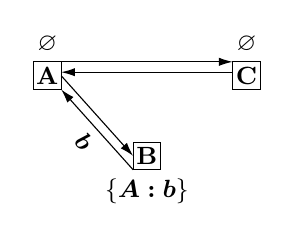
\begin{tikzpicture}[scale=1]
  
  \small
  
  \newcommand\X{180/5pt};
  \newcommand\Y{29pt};

  
  \draw[fill=white] (0*\X, 0*\Y) node{\textbf{A}} +(-5pt, -5pt) rectangle +(5pt, 5pt);
  \draw (0*\X, 5+0*\Y) node[above]{$\varnothing$};
  \draw[fill=white] (1*\X, -1*\Y) node{\textbf{B}} +(-5pt, -5pt) rectangle +(5pt, 5pt);
  \draw (1*\X, -5-1*\Y) node[below]{$\{\bm{A:b}\}$};
  \draw[fill=white] (2*\X,  0*\Y) node{\textbf{C}} +(-5pt, -5pt) rectangle +(5pt, 5pt);
  \draw (2*\X, 5+0*\Y) node[above]{$\varnothing$};
  
  \draw[->](5+0*\X, 0*\Y) --  (-5+1*\X, -1*\Y); %% A->B
  \draw[<-](5+0*\X, -5+0*\Y) -- node[sloped,below]{$\bm{b}$} (-5+1*\X, -5-1*\Y); %% A<-B
  
  \draw[->](5+0*\X, 5+0*\Y) -- (-5+2*\X, 5+0*\Y); % A->C
  \draw[<-](5+0*\X,  1.25+ 0*\Y) -- (-5+2*\X,  1.25+ 0*\Y); % A<-C
  
  % \draw[->,dashed](5+1*\X, -1*\Y) -- (-5+2*\X, 0*\Y); %% B<-C
  % \draw[->, dashed](5+1*\X, -5-1*\Y) -- (-5+2*\X, -5+0*\Y); %% B->C



\end{tikzpicture}%
      \caption{\label{fig:memorylinkA}Process~B broadcasts $b$ and awaits a copy
        of $b$ from Process~A.}
    \end{subfigure}
    ~
    \begin{subfigure}[t]{0.23\textwidth}
      \centering
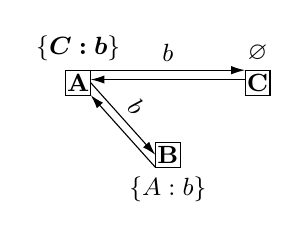
\begin{tikzpicture}[scale=0.9]
  
  \small
  
  \newcommand\X{180/5pt};
  \newcommand\Y{29pt};

  
  \draw[fill=white] (0*\X, 0*\Y) node{\textbf{A}} +(-5pt, -5pt) rectangle +(5pt, 5pt);
  \draw (0*\X, 5+0*\Y) node[above]{$\{\bm{C:b}\}$};
  \draw[fill=white] (1*\X, -1*\Y) node{\textbf{B}} +(-5pt, -5pt) rectangle +(5pt, 5pt);
  \draw (1*\X, -5-1*\Y) node[below]{$\{A:b\}$};
  \draw[fill=white] (2*\X,  0*\Y) node{\textbf{C}} +(-5pt, -5pt) rectangle +(5pt, 5pt);
  \draw (2*\X, 5+0*\Y) node[above]{$\varnothing$};
  
  \draw[->](5+0*\X, 0*\Y) -- 
  node[sloped,above]{$b$}
  (-5+1*\X, -1*\Y); %% A->B

  \draw[<-](5+0*\X, -5+0*\Y) -- (-5+1*\X, -5-1*\Y); %% A<-B
  
  \draw[->](5+0*\X, 5+0*\Y) --
  node[sloped,above]{$b$}
  (-5+2*\X, 5+0*\Y); % A->C
  
  \draw[<-](5+0*\X,  1.25+ 0*\Y) -- (-5+2*\X,  1.25+ 0*\Y); % A<-C
  
  % \draw[->,dashed](5+1*\X, -1*\Y) -- (-5+2*\X, 0*\Y); %% B<-C
  % \draw[->, dashed](5+1*\X, -5-1*\Y) -- (-5+2*\X, -5+0*\Y); %% B->C



\end{tikzpicture}%
      \caption{\label{fig:memorylinkB}Process~A receives, delivers, and forwards
        $b$. It expects a copy from Process~C.}
    \end{subfigure}
    ~
    \begin{subfigure}[t]{0.23\textwidth}
      \centering
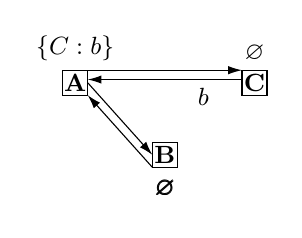
\begin{tikzpicture}[scale=0.9]
  
  \small
  
  \newcommand\X{180/5pt};
  \newcommand\Y{29pt};

  
  \draw[fill=white] (0*\X, 0*\Y) node{\textbf{A}} +(-5pt, -5pt) rectangle +(5pt, 5pt);
  \draw (0*\X, 5+0*\Y) node[above]{$\{C:b\}$};
  \draw[fill=white] (1*\X, -1*\Y) node{\textbf{B}} +(-5pt, -5pt) rectangle +(5pt, 5pt);
  \draw (1*\X, -5-1*\Y) node[below]{$\bm{\varnothing}$\vphantom{$\{$}};
  \draw[fill=white] (2*\X,  0*\Y) node{\textbf{C}} +(-5pt, -5pt) rectangle +(5pt, 5pt);
  \draw (2*\X, 5+0*\Y) node[above]{$\varnothing$};
  
  \draw[->](5+0*\X, 0*\Y) -- 
  (-5+1*\X, -1*\Y); %% A->B

  \draw[<-](5+0*\X, -5+0*\Y) --
  (-5+1*\X, -5-1*\Y); %% A<-B
  
  \draw[->](5+0*\X, 5+0*\Y) -- (-5+2*\X, 5+0*\Y); % A->C
  
  \draw[<-](5+0*\X,  1.25+ 0*\Y) --
  node[below]{ ~ ~ ~ ~ ~$b$}
 (-5+2*\X,  1.25+ 0*\Y); % A<-C
  
 % \draw[->,dashed](5+1*\X, -1*\Y) -- (-5+2*\X, 0*\Y); %% B<-C
 % \draw[->, dashed](5+1*\X, -5-1*\Y) -- (-5+2*\X, -5+0*\Y); %% B->C



\end{tikzpicture}%
      \caption{\label{fig:memorylinkC}Process~B and Process~C receive $b$. They
        do not expect additional copies. Process~C delivers and forwards $b$.}
    \end{subfigure}
    ~
    \begin{subfigure}[t]{0.23\textwidth}
      \centering
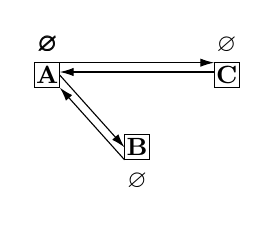
\begin{tikzpicture}[scale=0.9]
  
  \small
  
  \newcommand\X{180/5pt};
  \newcommand\Y{29pt};

  
  \draw[fill=white] (0*\X, 0*\Y) node{\textbf{A}} +(-5pt, -5pt) rectangle +(5pt, 5pt);
  \draw (0*\X, 5+0*\Y) node[above]{$\bm{\varnothing}$};
  \draw[fill=white] (1*\X, -1*\Y) node{\textbf{B}} +(-5pt, -5pt) rectangle +(5pt, 5pt);
  \draw (1*\X, -5-1*\Y) node[below]{$\varnothing$\vphantom{$\{$}};
  \draw[fill=white] (2*\X,  0*\Y) node{\textbf{C}} +(-5pt, -5pt) rectangle +(5pt, 5pt);
  \draw (2*\X, 5+0*\Y) node[above]{$\varnothing$};
  
  \draw[->](5+0*\X, 0*\Y) -- 
  (-5+1*\X, -1*\Y); %% A->B

  \draw[<-](5+0*\X, -5+0*\Y) --
  (-5+1*\X, -5-1*\Y); %% A<-B
  
  \draw[->](5+0*\X, 5+0*\Y) -- (-5+2*\X, 5+0*\Y); % A->C
  
  \draw[<-](5+0*\X,  1.25+ 0*\Y) --
 (-5+2*\X,  1.25+ 0*\Y); % A<-C
  
 % \draw[->,dashed](5+1*\X, -1*\Y) -- (-5+2*\X, 0*\Y); %% B<-C
 % \draw[->, dashed](5+1*\X, -5-1*\Y) -- (-5+2*\X, -5+0*\Y); %% B->C



\end{tikzpicture}%
      \caption{\label{fig:memorylinkD}Process~A receives its last expected copy
        of $b$. The message $b$ is completely removed from the system.}
    \end{subfigure}
    \caption{\label{fig:memorylink}Link memory allows processes to safely remove
      obsolete control information about past deliveries in static systems.}
  \end{center}
\end{figure}



%Vector clocks implement remembering but fail to remove obsolete control
%information. 

Algorithm~\ref{algo:reliablebroadcast} shows an implementation of uniform
reliable broadcast that uses link memory to forbid multiple delivery in static
systems. The link memory is non-monotonic. The first receipt of a broadcast
message from a link tags the other links (see Line~\ref{line:remembers}). The
receipt on other links of this broadcast message removes the corresponding tag
(see Line~\ref{line:forgets}). Figure~\ref{fig:memorylink} depicts its
functioning in a system comprising 3 processes. In Figure~\ref{fig:memorylinkA},
Process~B broadcasts $b$. It awaits a copy of $b$ from the only link in its
in-view. In Figure~\ref{fig:memorylinkB}, Process~A receives $b$. It delivers
it, for no link in its in-view is tagged with $b$, meaning this is a first
receipt. It tags the other link in its in-view with $b$ and forwards $b$ to its
out-view. In Figure~\ref{fig:memorylinkC}, Process~B receives the awaited copy
of $b$ from Process~A. It removes the corresponding entry. Process~B does not
consume space anymore for reliable broadcast. Process~C receives $b$. It detects
a first receipt so it delivers and forwards $b$. It does not tag any link, for
the only link from its in-view is the link from which it just received $b$. In
Figure~\ref{fig:memorylinkD}, the last process to await a copy of $b$ finally
receives it. None of processes remembers about $b$. No copy of $b$ travels in
the system. This implementation forbids multiple delivery in static systems.


\begin{figure}
  \begin{center}
    \begin{subfigure}[t]{0.23\textwidth}
      \centering
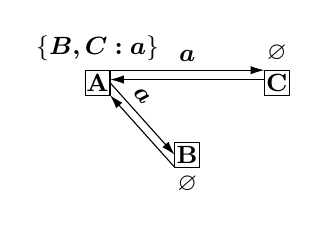
\begin{tikzpicture}[scale=0.9]
  
  \small
  
  \newcommand\X{180/5pt};
  \newcommand\Y{29pt};

  
  \draw[fill=white] (0*\X, 0*\Y) node{\textbf{A}} +(-5pt, -5pt) rectangle +(5pt, 5pt);
  \draw (0*\X, 5+0*\Y) node[above]{$\{\bm{B,C: a}\}$};
  \draw[fill=white] (1*\X, -1*\Y) node{\textbf{B}} +(-5pt, -5pt) rectangle +(5pt, 5pt);
  \draw (1*\X, -5-1*\Y) node[below]{$\varnothing$};
  \draw[fill=white] (2*\X,  0*\Y) node{\textbf{C}} +(-5pt, -5pt) rectangle +(5pt, 5pt);
  \draw (2*\X, 5+0*\Y) node[above]{$\varnothing$};
  
  \draw[->](5+0*\X, 0*\Y) --
  node[sloped, above]{$\bm{a}$~ ~ ~}
  (-5+1*\X, -1*\Y); %% A->B

  \draw[<-](5+0*\X, -5+0*\Y) -- 
  (-5+1*\X, -5-1*\Y); %% A<-B
  
  \draw[->](5+0*\X, 5+0*\Y) -- node[above]{$\bm{a}$} (-5+2*\X, 5+0*\Y); % A->C
  \draw[<-](5+0*\X,  1.25+ 0*\Y) -- (-5+2*\X,  1.25+ 0*\Y); % A<-C
  
  % \draw[->,dashed](5+1*\X, -1*\Y) -- (-5+2*\X, 0*\Y); %% B<-C
  % \draw[->, dashed](5+1*\X, -5-1*\Y) -- (-5+2*\X, -5+0*\Y); %% B->C



\end{tikzpicture}%
      \caption{\label{fig:memorylinkfailsA}Process~A broadcasts $a$ and expects a copy
        from both Process~B and Process~C.}
    \end{subfigure}
    ~
    \begin{subfigure}[t]{0.23\textwidth}
      \centering
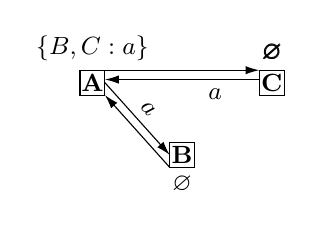
\begin{tikzpicture}[scale=0.9]
  
  \small
  
  \newcommand\X{180/5pt};
  \newcommand\Y{29pt};

  
  \draw[fill=white] (0*\X, 0*\Y) node{\textbf{A}} +(-5pt, -5pt) rectangle +(5pt, 5pt);
  \draw (0*\X, 5+0*\Y) node[above]{$\{B,C: a\}$};
  \draw[fill=white] (1*\X, -1*\Y) node{\textbf{B}} +(-5pt, -5pt) rectangle +(5pt, 5pt);
  \draw (1*\X, -5-1*\Y) node[below]{$\varnothing$};
  \draw[fill=white] (2*\X,  0*\Y) node{\textbf{C}} +(-5pt, -5pt) rectangle +(5pt, 5pt);
  \draw (2*\X, 5+0*\Y) node[above]{$\bm{\varnothing}$};
  
  \draw[->](5+0*\X, 0*\Y) --
  node[above, sloped]{$a$}
  (-5+1*\X, -1*\Y); %% A->B

  \draw[<-](5+0*\X, -5+0*\Y) -- 
  (-5+1*\X, -5-1*\Y); %% A<-B
  
  \draw[->](5+0*\X, 5+0*\Y) -- (-5+2*\X, 5+0*\Y); % A->C
  \draw[<-](5+0*\X,  1.25+ 0*\Y) -- node[below right]{ ~ $a$} (-5+2*\X,  1.25+ 0*\Y); % A<-C
  
  % \draw[->,dashed](5+1*\X, -1*\Y) -- (-5+2*\X, 0*\Y); %% B<-C
  % \draw[->, dashed](5+1*\X, -5-1*\Y) -- (-5+2*\X, -5+0*\Y); %% B->C



\end{tikzpicture}%
      \caption{\label{fig:memorylinkfailsB}Process C receives, delivers, and
        forwards $a$. It does not expect additional copies.}
    \end{subfigure}
    ~
    \begin{subfigure}[t]{0.23\textwidth}
      \centering
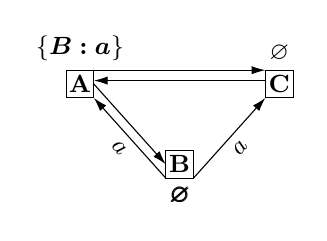
\begin{tikzpicture}[scale=1]
  
  \small
  
  \newcommand\X{180/5pt};
  \newcommand\Y{29pt};

  
  \draw[fill=white] (0*\X, 0*\Y) node{\textbf{A}} +(-5pt, -5pt) rectangle +(5pt, 5pt);
  \draw (0*\X, 5+0*\Y) node[above]{$\{\bm{B: a}\}$};
  \draw[fill=white] (1*\X, -1*\Y) node{\textbf{B}} +(-5pt, -5pt) rectangle +(5pt, 5pt);
  \draw (1*\X, -5-1*\Y) node[below]{$\bm{\varnothing}$};
  \draw[fill=white] (2*\X,  0*\Y) node{\textbf{C}} +(-5pt, -5pt) rectangle +(5pt, 5pt);
  \draw (2*\X, 5+0*\Y) node[above]{$\varnothing$};
  
  \draw[->](5+0*\X, 0*\Y) --
  (-5+1*\X, -1*\Y); %% A->B

  \draw[<-](5+0*\X, -5+0*\Y) -- 
  node[below, sloped]{$a$}
  (-5+1*\X, -5-1*\Y); %% A<-B
  
  \draw[->](5+0*\X, 5+0*\Y) -- (-5+2*\X, 5+0*\Y); % A->C
  \draw[<-](5+0*\X,  1.25+ 0*\Y) -- (-5+2*\X,  1.25+ 0*\Y); % A<-C
  
  % \draw[->,dashed](5+1*\X, -1*\Y) -- (-5+2*\X, 0*\Y); %% B<-C
  \draw[->](5+1*\X, -5-1*\Y) -- node[below, sloped]{$a$} (-5+2*\X, -5+0*\Y); %% B->C



\end{tikzpicture}%
      \caption{\label{fig:memorylinkfailsC}Process~B adds a link to Process~C. 
        Then it receives, delivers, and forwards $a$.}
    \end{subfigure}
    ~
    \begin{subfigure}[t]{0.23\textwidth}
      \centering
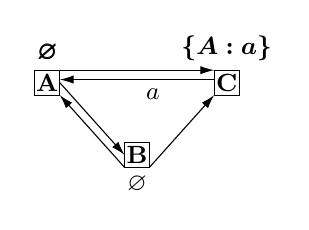
\begin{tikzpicture}[scale=0.9]
  
  \small
  
  \newcommand\X{180/5pt};
  \newcommand\Y{29pt};

  
  \draw[fill=white] (0*\X, 0*\Y) node{\textbf{A}} +(-5pt, -5pt) rectangle +(5pt, 5pt);
  \draw (0*\X, 5+0*\Y) node[above]{$\bm{\varnothing}$};
  \draw[fill=white] (1*\X, -1*\Y) node{\textbf{B}} +(-5pt, -5pt) rectangle +(5pt, 5pt);
  \draw (1*\X, -5-1*\Y) node[below]{$\varnothing$};
  \draw[fill=white] (2*\X,  0*\Y) node{\textbf{C}} +(-5pt, -5pt) rectangle +(5pt, 5pt);
  \draw (2*\X, 5+0*\Y) node[above]{$\bm{\{A:a\}}$};
  
  \draw[->](5+0*\X, 0*\Y) --
  (-5+1*\X, -1*\Y); %% A->B

  \draw[<-](5+0*\X, -5+0*\Y) -- 
  (-5+1*\X, -5-1*\Y); %% A<-B
  
  \draw[->](5+0*\X, 5+0*\Y) -- (-5+2*\X, 5+0*\Y); % A->C
  \draw[<-](5+0*\X,  1.25+ 0*\Y) -- node[below right]{$a$} (-5+2*\X,  1.25+ 0*\Y); % A<-C
  
  % \draw[->,dashed](5+1*\X, -1*\Y) -- (-5+2*\X, 0*\Y); %% B<-C
  \draw[->](5+1*\X, -5-1*\Y) -- (-5+2*\X, -5+0*\Y); %% B->C



\end{tikzpicture}%
      \caption{\label{fig:memorylinkfailsD}Process~C receives and mistakes $a$
        for a new message. It delivers, and forwards $a$.}
    \end{subfigure}
    \caption{\label{fig:memorylinkfails}Reliable broadcast
      (Algorithm~\ref{algo:reliablebroadcast}) fails to forbid multiple delivery
      in dynamic systems. }
  \end{center}
\end{figure}



However, implementing link memory becomes more challenging in dynamic systems
where processes can start sending messages to any other process at any time. Any
process can receive an already forgotten message from any other
process. Figure~\ref{fig:memorylinkfails} illustrates the issue. In
Figure~\ref{fig:memorylinkfailsA}, Process~A broadcasts $a$. It expects a copy
from both Process~B and Process~C. In Figure~\ref{fig:memorylinkfailsB},
Process~C immediately receives, delivers, and forwards $a$. It does not tag any
link and expects to never receive this message again. However, network condition
delays the receipt of $b$ from Process~B. In Figure~\ref{fig:memorylinkfailsC}
adds a communication link towards Process~C. Then it receives, delivers, and
forwards $b$. Since Process~C now belongs to its out-view, the forwarding
includes Process~C. In Figure~\ref{fig:memorylinkfailsD}, Process~C receives $a$
again. However, it did not keep control information about this message. It
mistakes it for a first receipt. It delivers and forwards $a$. Not only
Process~C suffers multiple delivery but this has cascading effects over the
whole system.

In this paper, we solve this issue by exploiting causal broadcast's ability to
ensure a specific order on message delivery. To characterize the order among
events such as send, or receive, we define time in a logical sense using
Lamport’s definition.

\begin{definition}[Happen before~\cite{lamport1978time}]
  Happen before is a transitive, irreflexive, and antisymmetric relation
  $\rightarrow$ that defines a strict partial orders of events. The sending of a
  message always precedes its receipt $s_{AB}(m) \rightarrow r_{BA}(m)$. Two
  messages are concurrent if none happens before the other.
\end{definition}

\begin{definition}[Causal order]
  The delivery order of messages follows the happen before relationships of the
  corresponding broadcasts.
  $d_A(m) \rightarrow b_A(m') \implies d_B(m) \rightarrow d_B(m')$
\end{definition}

\begin{definition}[Causal broadcast]
  Causal broadcast is a uniform reliable broadcast ensuring causal order.
\end{definition}

% \begin{figure}
%   \begin{center}
%     
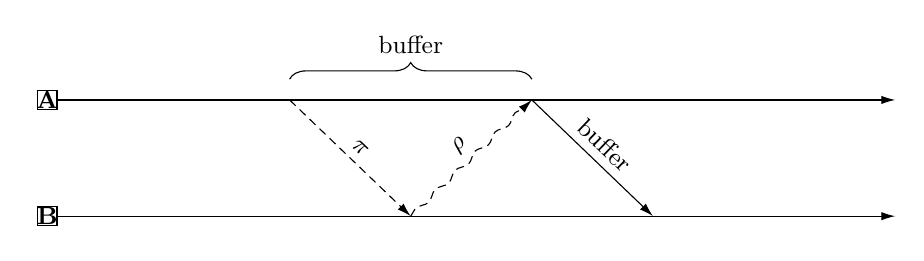
\begin{tikzpicture}[scale=0.7]

  \small
  
  \newcommand\X{1.45*\columnwidth/8pt};
  \newcommand\YA{0pt};
  \newcommand\YB{-60pt};


  \draw[->](2*\X, \YA) -- (9*\X, \YA);
  \draw[->](2*\X, \YB) -- (9*\X, \YB);
  
  \draw[fill=white] (2*\X, \YA) node{\textbf{\textup{A}}}
  +(-5pt, -5pt) rectangle +(5pt, 5pt);
  \draw[fill=white] (2*\X, \YB)  node{\textbf{\textup{B}}}
  +(-5pt, -5pt) rectangle +(5pt, 5pt);

  % \draw ( 1*\X, \YA ) node[above]{$\mathcal{A}$};
  % \draw ( 1*\X, \YB ) node[below]{$\mathcal{B}$};

%  \draw[->] ( 2*\X, \YA ) -- node[sloped, above]{$\alpha$} (3*\X, \YB);
  % node[below left]{$\mathcal{A}$};

  % \draw[decorate,decoration={brace,amplitude=6pt,mirror,raise=4pt}] (3*\X,
  % -5+\YB) -- node[anchor=north, yshift=-10pt]{$B_{B\alpha}$}
  % (5*\X, -5+\YB);

  % \draw ( 3*\X, \YA ) node[above]{$\mathcal{C}$};

  % \draw[->] ( 3*\X, \YB ) -- node[sloped, above]{$\beta$} (4*\X, \YA);
  % node[above left]{$\mathcal{B}$};

  \draw[decorate,decoration={brace,amplitude=6pt,raise=4pt}] 
  (4*\X, 5+\YA) 
  -- node[anchor=south, yshift=10pt]{buffer}
  (6*\X, 5+\YA);

  % \draw[decorate,thick,decoration={brace,amplitude=6pt,raise=4pt}] (6*\X,
  % 5+\YA) -- node[anchor=south, yshift=10pt]{$\bm{B_{A\pi}}$}
  % (8*\X, 5+\YA);
  
  
  % \draw ( 4*\X, \YB ) node[below]{$\mathcal{D}$};

  \draw[->, densely dashed] ( 4*\X, \YA ) -- node[sloped, above]{$\pi$} (5*\X, \YB);
  % node[below left]{$\mathcal{C}$};

  % \draw[decorate,decoration={brace,amplitude=6pt,mirror,raise=4pt}] (5*\X,
  % -5+\YB) -- node[anchor=north, yshift=-10pt]{$B_{B\pi} \bm{= B_{B\beta}}$}
  % (7*\X, -5+\YB);


  % \draw ( 5*\X, \YA ) node[above]{$\mathcal{E}$};

  \draw[->, densely dashed, decorate, decoration={snake, amplitude=0.3mm}] ( 5*\X, \YB ) -- node[sloped, above]{$\rho$} (6*\X, \YA);
  % node[above left]{$\mathcal{D}$};
  
  % \draw (6*\X, \YB) node[below]{$\mathcal{F}$};

  \draw[->] ( 6*\X, \YA ) -- node[sloped, above]{buffer} (7*\X, \YB);

  % \draw[->, dashed, thick] ( 7*\X, \YB ) --
  % node[sloped, below]{$\bm{B_{B\beta}}$} (8*\X, \YA);

%  node[below left]{$\mathcal{E}$};


\end{tikzpicture}

%%% Local Variables:
%%% mode: latex
%%% TeX-master: "../paper"
%%% End:

%     \caption{\label{fig:timelinepcbroadcast}Process~A ensures the safety of a
%       link to Process~B. $\pi$ travels using safe links through intermediary
%       processes that are hidden for the sake of clarity. $\rho$ reaches
%       Process~A by any communication mean. Process~A sends the array of buffered
%       messages via the new link. The link becomes safe.}
%   \end{center}
% \end{figure}

% \begin{problem*}
%   Figure~\ref{fig:problemstatement} depicts this problem. Assuming Process~A
%   sends a buffer of messages to Process~B in order to finalize the safety of
%   this link. Upon receipt of this buffer by Process~B, the scientific problem
%   consists in:
%   \begin{itemize}[leftmargin=*]
%   \item Identifying the array of messages from the buffer that are delivered by
%     Process~A but not delivered by Process~B in order to deliver them;
%   \item Identifying the set of messages from the buffer that are delivered by
%     Process~A and Process~B in order to forget them;
%   \item Identifying the set of messages delivered by Process~B that Process~B will
%     receive by this safe link in order to remember them.
%   \end{itemize}%
% %  These are the array of messages to deliver, the set of messages to ignore, and
% %  the set of messages to expect, respectively.
% \end{problem*}

% \begin{figure}
%   \begin{center}
%     
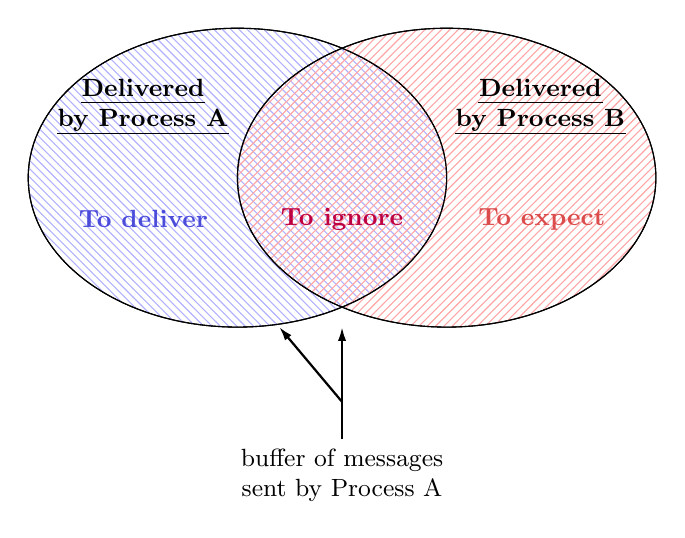
\begin{tikzpicture}[scale=1]

  \small
  
  \newcommand\X{210/5pt};
  \newcommand\Y{30pt};
  
  \newcommand\RADX{1.8};
  \newcommand\RADY{1.8};

  \newcommand\OFFX{15pt};

  \draw[->, thick] (0.5*\RADX*\X, -1.75*\RADY*\Y) node[below, align=center]{buffer of messages\\sent by Process~A} -- (0.5*\RADX*\X, -1*\RADY*\Y);
  \draw[->, thick] (0.5*\RADX*\X, -1.5*\RADY*\Y) -- (0.2*\RADX*\X, -1*\RADY*\Y);
%  \draw[->, thick] (0.5*\RADX*\X, -1.5*\RADY*\Y) -- node[sloped]{\Large$\times$} (0.8*\RADX*\X, -1*\RADY*\Y);
  
  \draw[pattern=north west lines, pattern color=blue!30] (0*\X, 0pt) circle [x radius=\RADX*\X, y radius = \RADY*\Y];
  \draw[pattern=north east lines, pattern color=red!35] (\RADX*\X, 0pt) circle [x radius=\RADX*\X, y radius = \RADY*\Y];
  \draw (\RADX*\X, 0pt) circle [x radius=\RADX*\X, y radius = \RADY*\Y];
  \draw (0*\X, 0pt) circle [x radius=\RADX*\X, y radius = \RADY*\Y];

  \draw (0*\X, -\OFFX+\RADY*\Y) node[below left, align=center]
  {\textbf{\uline{Delivered}}\\\textbf{\uline{by Process~A}}};

  \draw (\OFFX-\RADX*\X, -\OFFX+0pt) node[right, align=left] {
    \textbf{\COLOR{blue!80!black!70}{To deliver}}%\tiny
    % $B_\beta \setminus B_\alpha \setminus B_\pi$\\%\tiny
    % $[b_1,\,b_2,\,c_2]\setminus\{c_1,\,c_2\}\setminus\{b_1,\,c_3\}$\\%\tiny
    % $[b_1,\,b_2] \setminus \{b_1,\,c_3\}$\\%\tiny
    % $[b_2]$
  };
  \draw (-\OFFX+2*\RADX*\X, -\OFFX+0pt) node[left, align=right] {
    \textbf{\COLOR{red!80!black!70}{To expect}}%\tiny
    % $B_\pi \setminus (B_\beta \setminus B_\alpha)$\\%\tiny
    % $\{b_1,\,c_3\} \setminus ([b_1,\,b_2,\,c_2] \setminus\{c_1,\,c_2\})$\\%\tiny
    % $\{b_1,\,c_3\} \setminus [b_1,\,b_2]$\\%\tiny
    % $\{c_3\}$
  };
  \draw (0.5*\RADX*\X, -\OFFX+0pt) node[align=center] {
    \textbf{\COLOR{purple}{To ignore}}%\tiny
    % $B_\beta \setminus B_\alpha \wedge B_\pi$\\%\tiny
    % $[b_1,\,b_2,\,c_2] \setminus \{c_1,\,c_2\} \wedge \{ b_1,\,c_3\}$\\%\tiny
    % $[b_1,\,b_2] \wedge \{ b_1, \, c_3 \}$\\%\tiny
    % $\{ b_1 \}$
  };
  \draw (\RADX*\X, -\OFFX+\RADY*\Y) node[below right, align=center]
  {\textbf{\uline{Delivered}}\\\textbf{\uline{by Process~B}}};


\end{tikzpicture}

%     \caption{\label{fig:problemstatement}For each message in the buffer,
%       Process~B must identify its category and assign awaited messages on the
%       new safe link.}
%   \end{center}
% \end{figure}

The rest of this section describes how reliable broadcast can exploit causal
order to initialize safe link memory. Then, we provide an implementation of such
broadcast along with its complexity analysis.

\subsection{Principle}

This section demonstrates that reliable broadcast can use causal order brought
by causal broadcast to initialize safe link memory, hence provide a
non-monotonic local structure that removes all and only obsolete information in
large and dynamic systems.

Figure~\ref{fig:memorylink} shows that Algorithm~\ref{algo:reliablebroadcast}
already implements the maintenance of link memory over receipts. Processes
discard obsolete control information over receipts.  However,
Figure~\ref{fig:memorylinkfails} shows that new links lack of consistent
initialization. The challenge consists in initializing such memory without
history of past messages. Causal broadcast starts to build the knowledge
on-demand, i.e., when a process wants to add a link to another process.  The
protocol disables the new link until it is initialized. This initialization
requires round-trips of control messages and message buffering.  Causal
broadcast takes advantage of causal order to provide guarantees on messages
included in buffers.

% \begin{figure*}
%   \begin{center}
%     
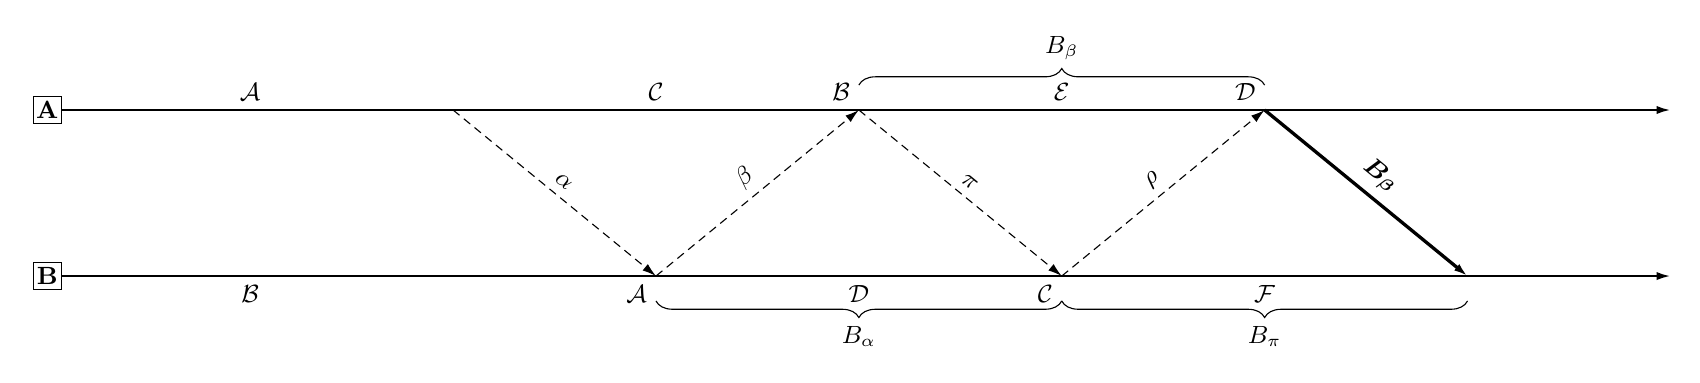
\begin{tikzpicture}[scale=1]

  \small
  
  \newcommand\X{1.7*\columnwidth/8pt};
  \newcommand\YA{0pt};
  \newcommand\YB{-60pt};


  \draw[->, thick](0*\X, \YA) -- (8*\X, \YA);
  \draw[->, thick](0*\X, \YB) -- (8*\X, \YB);
  
  \draw[fill=white] (0*\X, \YA) node{\textbf{\textup{A}}} +(-5pt, -5pt) rectangle +(5pt, 5pt);
  \draw[fill=white] (0*\X, \YB) node{\textbf{\textup{B}}} +(-5pt, -5pt) rectangle +(5pt, 5pt);

  \draw ( 1*\X, \YA ) node[above]{$\mathcal{A}$};
  \draw ( 1*\X, \YB ) node[below]{$\mathcal{B}$};

  \draw[densely dashed,->] ( 2*\X, \YA ) -- node[sloped, above]{$\alpha$} (3*\X, \YB)
  node[below left]{$\mathcal{A}$};

  \draw[decorate,decoration={brace,amplitude=6pt,mirror,raise=4pt}] (3*\X,
  -5+\YB) -- node[anchor=north, yshift=-10pt]{$B_\alpha$}
  (5*\X, -5+\YB);

  \draw ( 3*\X, \YA ) node[above]{$\mathcal{C}$};

  \draw[densely dashed,->] ( 3*\X, \YB ) -- node[sloped, above]{$\beta$} (4*\X, \YA)
  node[above left]{$\mathcal{B}$};

  \draw[decorate,decoration={brace,amplitude=6pt,raise=4pt}] (4*\X,
  5+\YA) -- node[anchor=south, yshift=10pt]{$B_\beta$}
  (6*\X, 5+\YA);
  
  
  \draw ( 4*\X, \YB ) node[below]{$\mathcal{D}$};

  \draw[densely dashed,->] ( 4*\X, \YA ) -- node[sloped, above]{$\pi$} (5*\X, \YB)
  node[below left]{$\mathcal{C}$};

  \draw[decorate,decoration={brace,amplitude=6pt,mirror,raise=4pt}] (5*\X,
  -5+\YB) -- node[anchor=north, yshift=-10pt]{$B_\pi$}
  (7*\X, -5+\YB);


  \draw ( 5*\X, \YA ) node[above]{$\mathcal{E}$};

  \draw[densely dashed,->] ( 5*\X, \YB ) -- node[sloped, above]{$\rho$} (6*\X, \YA)
  node[above left]{$\mathcal{D}$};
  
  \draw (6*\X, \YB) node[below]{$\mathcal{F}$};

  \draw[->, very thick] ( 6*\X, \YA ) -- node[sloped, above]{$\bm{B_\beta}$} (7*\X, \YB);
%  node[below left]{$\mathcal{E}$};


\end{tikzpicture}

%%% Local Variables:
%%% mode: latex
%%% TeX-master: "../paper"
%%% End:

%     \caption{\label{fig:timeline}Timeline of \RPCBROADCAST when Process~A adds a
%       link to Process~B in its out-view. We hide intermediate processes for the
%       purpose of clarity. Messages arrive in causal order.}
%   \end{center}
% \end{figure*}

Figure~\ref{fig:timelineproof} depicts the principle of the approach. When a
Process~A adds a link to
Process~B. %, \RPCBROADCAST initializes safe link memory
% in 3 steps.
Process~A notifies Process~B using a control message $\alpha$. This control
message $\alpha$, as all control messages that will follow ($\beta$, $\pi$,
$\rho$), are delivered in causal order regarding broadcast messages. Hence, at
receipt, Process~B implicitly removes obsolete information: messages delivered
by Process~A before the sending of the notification $\mathcal{A}_1$. 
At receipt
of $\alpha$, Process~B can start gathering control information about its
delivered messages in a buffer $B_\alpha$. Among other, Process~B wants to
identify messages concurrent to the correct establishment of the new
link. Process~B acknowledges Process~A's notification using a control message
$\beta$. At receipt of $\beta$, Process~A removes obsolete information: messages
delivered by Process~B before the sending of the acknowledgment
$\mathcal{A}_1 \cup \mathcal{B}_1$. This solves the issue
identified in Figure~\ref{fig:memorylinkfails}, for $a$ would belong to $\mathcal{A}_1$
or $\mathcal{B}_1$. However, this is not sufficient to initialize link memory.
Process~A sends a control message $\pi$ to
Process~B, and starts to gather control information about its delivered messages
in a buffer $B_\beta$. Upon receipt of $\pi$, Process~B closes its first buffer
$B_\alpha$.

\begin{figure}
  \begin{center}
    
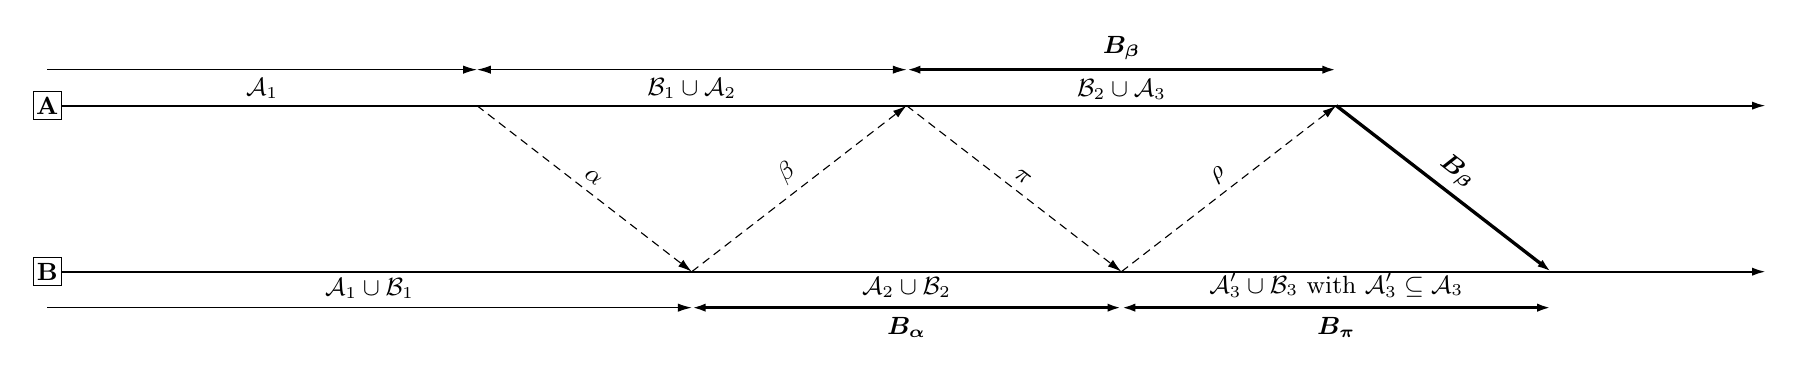
\begin{tikzpicture}[scale=1]

  \small
  
  \newcommand\X{1.8*\columnwidth/8pt};
  \newcommand\YA{0pt};
  \newcommand\YB{-60pt};
  
  \newcommand\YSPACE{13pt};

  \draw[->, thick](0*\X, \YA) -- (8*\X, \YA);
  \draw[->, thick](0*\X, \YB) -- (8*\X, \YB);
  
  \draw[fill=white] (0*\X, \YA) node{\textbf{\textup{A}}} +(-5pt, -5pt) rectangle +(5pt, 5pt);
  \draw[fill=white] (0*\X, \YB) node{\textbf{\textup{B}}} +(-5pt, -5pt) rectangle +(5pt, 5pt);
  
  \draw[->] (0*\X, \YA + 1* \YSPACE)% node[above right]{$\mathcal{A}$}
  -- node[below]{$\mathcal{A}_1$} (2*\X, \YA + \YSPACE);
  \draw[densely dashed,->] ( 2*\X, \YA ) -- node[sloped, above]{$\alpha$} (3*\X, \YB);

  \draw[->] (0*\X, \YB - 1* \YSPACE)
  %node[below right]{$\mathcal{B} = \mathcal{A} \cup \mathcal{A}'$} 
  -- node[above]{$\mathcal{A}_1 \cup \mathcal{B}_1$}
  (3*\X, \YB - \YSPACE);

  \draw[densely dashed,->] ( 3*\X, \YB ) -- node[sloped, above]{$\beta$} (4*\X, \YA);


  \draw[<->] ( 2*\X, \YA + 1* \YSPACE ) --
  node[below]{$\mathcal{B}_1 \cup \mathcal{A}_2$}
  (4*\X, \YA + 1* \YSPACE);
  % \draw[->] (0*\X, \YA + 2* \YSPACE)
  % node[above right]{$\mathcal{C} = \mathcal{B} \cup \mathcal{B}' = \mathcal{A} \cup \mathcal{A}' \cup \mathcal{B}'$} --
  % (4*\X, \YA + 2*\YSPACE);
  
  \draw[densely dashed,->] ( 4*\X, \YA ) -- node[sloped, above]{$\pi$} (5*\X, \YB);

  % \draw[->] (0*\X, \YB - 2 * \YSPACE)
  % node[below right]{$\mathcal{D} = \mathcal{C} \cup \mathcal{C}' = \mathcal{A} \cup \mathcal{A}' \cup \mathcal{B}' \cup \mathcal{C}'$} --
  % (5*\X, \YB - 2*\YSPACE);

  \draw[<->,very thick] (3*\X, \YB - 1*\YSPACE) --
  node[below]{$\bm{B_\alpha}$}
  node[above]{$\mathcal{A}_2 \cup \mathcal{B}_2$}
  (5*\X, \YB - 1*\YSPACE);

  \draw[densely dashed,->] ( 5*\X, \YB ) -- node[sloped, above]{$\rho$} (6*\X, \YA);

  % \draw[->] (0*\X, \YA + 3 * \YSPACE)
  % node[above right]{$\mathcal{E} = \mathcal{D} \cup \mathcal{D}' = \mathcal{A} \cup \mathcal{A}' \cup \mathcal{B}' \cup \mathcal{C}' \cup \mathcal{D}'$} --
  % (6*\X, \YA + 3*\YSPACE);

  \draw[<->,very thick] (4*\X, \YA +1*\YSPACE) -- node[above]{$\bm{B_\beta}$}
  node[below]{$\mathcal{B}_2 \cup \mathcal{A}_3$} (6*\X, \YA + 1*\YSPACE);


  \draw[->, very thick] ( 6*\X, \YA ) -- node[sloped, above]{$\bm{B_\beta}$} (7*\X, \YB);

  
  \draw[<->,very thick] (5*\X, \YB - 1*\YSPACE ) -- node[below]{$\bm{B_\pi}$}
  node[above]{$\mathcal{A}_3' \cup \mathcal{B}_3$ with
    $\mathcal{A}_3' \subseteq \mathcal{A}_3$} 
  (7*\X, \YB - 1*\YSPACE);


  % \draw[<-] (7*\X, -2+\YB ) -- (7.1*\X, \YB -  2*\YSPACE )
  % node[right, align=center]{$B_\beta\setminus B_\alpha \setminus B_\pi = \mathcal{D}' \setminus (\mathcal{G} \cup \mathcal{H}) = \mathcal{D}' \setminus \mathcal{G}$\\
  % $B_\pi \setminus (B_\beta \setminus B_\alpha) = (\mathcal{G} \cup \mathcal{H}) \setminus \mathcal{D}' = \mathcal{H} $\\
  % $B_\beta \setminus B_\alpha \wedge B_pi = \mathcal{D}' \wedge (\mathcal{G} \cup \mathcal{H}) = \mathcal{G}$};

\end{tikzpicture}

%%% Local Variables:
%%% mode: latex
%%% TeX-master: "../paper"
%%% End:

    \caption{\label{fig:timelineproof}\label{fig:timeline}Initializing the link
      memory from Process~A to Process~B. Control messages $\alpha$, $\beta$,
      $\pi$, and $\rho$ are delivered in causal order while $B_\beta$ is not.
      $B_\beta \cap (B_\alpha \cup B_\pi) = \mathcal{B}_2 \cup \mathcal{A}_3'$
      are messages to ignore;
      $B_\beta \setminus B_\alpha \setminus B_\pi = \mathcal{A}_3\setminus
      \mathcal{A}_3'$
      are messages to deliver; $B_\pi \setminus B_\beta = \mathcal{B}_3$ are
      messages to expect.}
  \end{center}
\end{figure}

  
\begin{lemma}[\label{lem:balpha}Messages in buffer $B_\alpha$]
  The buffer $B_\alpha$ contains messages delivered by Process~B after the
  sending of $\beta$ and before the receipt of $\pi$.\\
  This includes all messages delivered by Process~A before the sending of $\pi$
  that were not delivered by Process~B before the sending of $\beta$:
  $\mathcal{A}_2$. Most importantly, this also includes all messages delivered
  by Process~B that were not delivered by Process~A at the sending of $\pi$:
  $\mathcal{B}_2$.
\end{lemma}

\begin{proof}
  Since causal broadcast ensures causal order among messages it conveys, all
  messages delivered by Process~A before the sending of $\alpha$ precede the
  buffering:
  $\forall m,\, d_A(m) \rightarrow s_A(\alpha_{AB}) \implies m \not \in
  B_\alpha$.
  Since messages are delivered once,
  $\forall m,\, d_A(m) \rightarrow s_A(\pi_{AB}) \wedge d_B(m) \rightarrow
  s_B(\beta_{AB}) \implies m \not \in B_\alpha$.
  This removes $\mathcal{A}_1$ and $\mathcal{B}_1$.\\
  The buffer $B_\alpha$ contains the rest of messages delivered by Process~B
  before the receipt of $\pi$. This includes messages delivered by Process~A
  between the sending of $\alpha$ and $\pi$ but not delivered by Process~B
  before the sending of $\beta$ ($\mathcal{A}_2$); and messages delivered by
  Process~B but not delivered by Process~A before the sending of $\pi$
  ($\mathcal{B}_2$).
\end{proof}

\noindent Upon receipt of $\pi$, Process~B continues to gather control information about
its delivered messages in another buffer $B_\pi$. Some messages in this buffer
will be expected from Process~A, but Process~B cannot determine which ones just
yet. It sends the last acknowledgment $\rho$ to Process~A. Upon receipt of this
acknowledgment, Process~A closes its buffer and sends it using the new
link. Afterwards, Process~A uses the new link for causal broadcast, for it knows
that Process~B will receive $B_\beta$ before upcoming broadcast messages on this
new link, and the receipt of $B_\beta$ will allow Process~B to initialize this
new link memory.

\begin{lemma}[\label{lem:bbeta}Messages in buffer $B_\beta$]
  The buffer $B_\beta$ contains messages delivered by Process~A after the
  sending of $\pi$ and before the receipt of $\rho$.\\
  This includes all messages delivered by Process~B before the sending of
  $\rho$ that were not delivered by Process~A before the sending of $\pi$:
  $\mathcal{B}_2$. This also includes all messages delivered by Process~A that
  were not delivered by Process~B at the sending of $\rho$: $\mathcal{A}_3$.
\end{lemma}
  
\begin{proof}
  The proof is similar to that of Lemma~\ref{lem:balpha}. Control messages
  shift roles. $\pi$ becomes $\rho$; $\beta$ becomes $\pi$; $\alpha$ becomes
  $\beta$.
\end{proof}

\noindent Upon receipt of $B_\beta$, Process~B stops buffering in $B_\pi$.
  
\begin{lemma}[\label{lem:bpi}Messages in buffer $B_\pi$]
  The buffer $B_\pi$ contains messages delivered by Process~B after the
  sending of $\pi$ and before the receipt of $B_\beta$.\\
  This may includes messages delivered by Process~A before the sending of
  $B_\beta$ that were not delivered by Process~B before the sending of $\rho$:
  $\mathcal{A}_3'$. This also includes all messages delivered by Process~B that
  were not delivered by Process~A at the sending of $B_\beta$:
  $\mathcal{B}_3$. 
\end{lemma}

\begin{proof}
  The proof is similar to that of Lemmas~\ref{lem:bbeta}~and~\ref{lem:bpi}. The
  difference being that $B_\beta$ is not causally delivered. Hence, the receipt
  of $B_\beta$ follows the sending of $\rho$ but Process~B cannot state if it
  received all, part, or none of messages in $\mathcal{A}_3$. Thus,
  $\mathcal{A}_3' \subseteq \mathcal{A}_3$.
\end{proof}

\noindent Using $B_\alpha$, $B_\beta$, and $B_\pi$ buffers, Process~B identifies
messages in $B_\beta$ it must deliver against messages it must ignore, and
messages in $B_\pi$ it must receive from Process~A. This allows Process~B to
initialize link memory.

\begin{theorem}[$B_\alpha$, $B_\beta$, and $B_\pi$ build link memory]
  The memory of a new link becomes correct at receipt of $B_\beta$.
\end{theorem}

\begin{proof}
  From Lemma~\ref{lem:balpha}, $B_\alpha = \mathcal{A}_2 \cup \mathcal{B}_2$.
  From Lemma~\ref{lem:bbeta}, $B_\beta= \mathcal{B}_2 \cup \mathcal{A}_3$. From
  Lemma~\ref{lem:bpi}, $B_\pi = \mathcal{A}_3' \cup \mathcal{B}_3$. \\ First,
  for the maintenance of link memory, we must show that Process~B delivers all
  and only messages from $B_\beta$ it did not deliver yet:
  $\mathcal{A}_3 \setminus \mathcal{A}_3'$. Since
  $B_\beta \setminus B_\alpha \setminus B_\pi = (\mathcal{B}_2 \cup
  \mathcal{A}_3) \setminus (\mathcal{A}_2 \cup \mathcal{B}_2) \setminus
  (\mathcal{A}_3' \cup \mathcal{B}_3) = \mathcal{A}_3 \setminus \mathcal{A}_3'
  \cup \mathcal{B}_3 = \mathcal{A}_3'\setminus \mathcal{A}_3$
  (since $\mathcal{B}_3 \cap \mathcal{A}_3 = \varnothing$), Process~B identifies
  the set of messages to deliver using $B_\alpha$, $B_\beta$, and $B_\pi$. \\
  Second, for the initialization of link memory, we must show that Process~B
  initializes the new link memory with all and only messages from $B_\pi$ that
  Process~A did not deliver at the sending of $B_\beta$:
  $m \in \mathcal{B}_3 \Leftrightarrow d_B(m) \neg r_{BA}(m)$ and
  $m \in \mathcal{B}_3 \implies r_{BA}(m)$.  Since
  $B_\pi \cap B_\alpha = \varnothing$,
  $B_\pi \setminus (B_\beta \setminus B_\alpha)= B_\pi \setminus B_\beta =
  (\mathcal{A}_3' \cup \mathcal{B}_3) \setminus (\mathcal{B}_2 \cup
  \mathcal{A}_3) = \mathcal{B}_3$
  (since $\mathcal{B}_3 \cap \mathcal{B}_2 = \varnothing$ and
  $\mathcal{A}_3' \subseteq \mathcal{A}_3$), Process~B identifies the set of
  messages to await from Process~A using $B_\pi$ and $B_\beta$. This is the new
  link memory.
\end{proof}

\subsection{Implementation}

\RPCBROADCAST stands for Preventive Reliable Causal broadcast. It prevents
causal order violation and multiple delivery by using all and only links that
\begin{inparaenum}[(i)]
\item have been proven safe to use and
\item the memory of which is correctly initialized and maintained.
\end{inparaenum}
This guarantees causal order and non-monotonic local data structure in large and
dynamic systems. 

%% Table~\ref{table:complexity} shows that it keeps constant size message overhead
%% while discarding local control information about messages over receipts.

To provide causal order at marginal cost, \RPCBROADCAST uses the principle of
\PCBROADCAST~\cite{nedelec2018pcbroadcast}. It uses FIFO links, gossiping,
control messages, and buffers to ensure causal order in dynamic systems. A
process broadcasting a message sends the message to an out-view of safe links
that cannot lead to causal order violations. \RPCBROADCAST embeds safe link
establishment in its link memory initialization.

\begin{figure}
  \begin{center}
    \begin{subfigure}[t]{0.31\textwidth}
      \centering
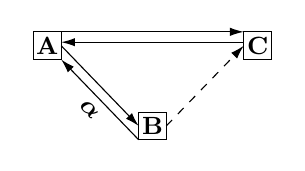
\begin{tikzpicture}[scale=1]
  
  \small
  
  \newcommand\X{190/5pt};
  \newcommand\Y{29pt};

  
  \draw[fill=white] (0*\X, 0*\Y) node{\textbf{A}} +(-5pt, -5pt) rectangle +(5pt, 5pt);
  % \draw (-5+0*\X, 0*\Y) node[left]{$E: \{a:2\}$};
  \draw[fill=white] (1*\X, -1*\Y) node{\textbf{B}} +(-5pt, -5pt) rectangle +(5pt, 5pt);
  % \draw (1*\X, -5-1*\Y) node[below]{$E: \varnothing$\vphantom{$\{$}};
  \draw[fill=white] (2*\X,  0*\Y) node{\textbf{C}} +(-5pt, -5pt) rectangle +(5pt, 5pt);
  % \draw (5+2*\X, 0*\Y) node[right]{$E: \varnothing$\vphantom{$\{$}};
  % \draw (5+2*\X, 0*\Y) node[right]{\phantom{$E: \{a:1\}$}};
  
  \draw[->](5+0*\X, 0*\Y) -- (-5+1*\X, -1*\Y); %% A->B
  \draw[<-](5+0*\X, -5+0*\Y) -- node[sloped, below]{$\bm{\alpha}$} (-5+1*\X, -5-1*\Y); %% A<-B
  
  \draw[->](5+0*\X, 5+0*\Y) -- (-5+2*\X, 5+0*\Y); % A->C
  \draw[<-](5+0*\X,  1.25+ 0*\Y) -- (-5+2*\X,  1.25+ 0*\Y); % A<-C
  
  \draw[->,dashed](5+1*\X, -1*\Y) -- (-5+2*\X, 0*\Y); %% B<-C
  % \draw[->, dashed](5+1*\X, -5-1*\Y) -- (-5+2*\X, -5+0*\Y); %% B->C



\end{tikzpicture}%
      \caption{\label{fig:solveA}Process~B adds a link to
        Process~C. \RPCBROADCAST ensures its safety. Process~B sends a first
        control message $\alpha$ to Process~C using Process~A as mediator.}
    \end{subfigure}
    ~
    \begin{subfigure}[t]{0.31\textwidth}
      \centering
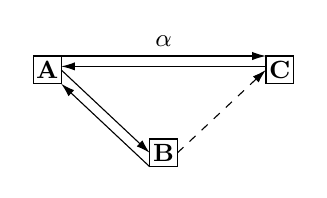
\begin{tikzpicture}[scale=1]
  
  \small
  
  \newcommand\X{210/5pt};
  \newcommand\Y{30pt};

  
  \draw[fill=white] (0*\X, 0*\Y) node{\textbf{A}} +(-5pt, -5pt) rectangle +(5pt, 5pt);
  % \draw (-5+0*\X, 0*\Y) node[left]{$E: \{a:2\}$};
  \draw[fill=white] (1*\X, -1*\Y) node{\textbf{B}} +(-5pt, -5pt) rectangle +(5pt, 5pt);
  % \draw (1*\X, -5-1*\Y) node[below]{$E: \varnothing$\vphantom{$\{$}};
  \draw[fill=white] (2*\X,  0*\Y) node{\textbf{C}} +(-5pt, -5pt) rectangle +(5pt, 5pt);
  % \draw (5+2*\X, 0*\Y) node[right]{$E: \varnothing$\vphantom{$\{$}};
  % \draw (5+2*\X, 0*\Y) node[right]{\phantom{$E: \{a:1\}$}};
  
  \draw[->](5+0*\X, 0*\Y) -- (-5+1*\X, -1*\Y); %% A->B
  \draw[<-](5+0*\X, -5+0*\Y) -- (-5+1*\X, -5-1*\Y); %% A<-B
  
  \draw[->](5+0*\X, 5+0*\Y) -- node[sloped, above]{$\alpha$} (-5+2*\X, 5+0*\Y); % A->C
  \draw[<-](5+0*\X,  1.25+ 0*\Y) -- (-5+2*\X,  1.25+ 0*\Y); % A<-C
  
  \draw[->,dashed](5+1*\X, -1*\Y) -- (-5+2*\X, 0*\Y); %% B<-C
  % \draw[->, dashed](5+1*\X, -5-1*\Y) -- (-5+2*\X, -5+0*\Y); %% B->C



\end{tikzpicture}%
      \caption{\label{fig:solveB}Process~A receives $\alpha$ and routes it to
        Process~C.}
    \end{subfigure}
    ~
    \begin{subfigure}[t]{0.31\textwidth}
      \centering
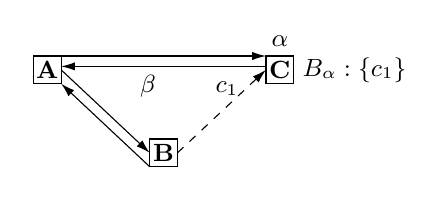
\begin{tikzpicture}[scale=1]
  
  \small
  
  \newcommand\X{210/5pt};
  \newcommand\Y{30pt};

  
  \draw[fill=white] (0*\X, 0*\Y) node{\textbf{A}} +(-5pt, -5pt) rectangle +(5pt, 5pt);
  % \draw (-5+0*\X, 0*\Y) node[left]{$E: \{a:2\}$};
  \draw[fill=white] (1*\X, -1*\Y) node{\textbf{B}} +(-5pt, -5pt) rectangle +(5pt, 5pt);
  % \draw (1*\X, -5-1*\Y) node[below]{$E: \varnothing$\vphantom{$\{$}};
  \draw[fill=white] (2*\X,  0*\Y) node{\textbf{C}} +(-5pt, -5pt) rectangle +(5pt, 5pt);
  \draw(2*\X, 5+0*\Y) node[above]{$\alpha$};
  \draw (5+2*\X, 0*\Y) node[right]{$B_\alpha: \{c_1\}$};
  % \draw (5+2*\X, 0*\Y) node[right]{\phantom{$E: \{a:1\}$}};
  
  \draw[->](5+0*\X, 0*\Y) -- (-5+1*\X, -1*\Y); %% A->B
  \draw[<-](5+0*\X, -5+0*\Y) -- (-5+1*\X, -5-1*\Y); %% A<-B
  
  \draw[->](5+0*\X, 5+0*\Y) -- (-5+2*\X, 5+0*\Y); % A->C
  \draw[<-](5+0*\X,  1.25+ 0*\Y) -- node[below]{~~~~~~$\beta$~~~~~~~$c_1$} (-5+2*\X,  1.25+ 0*\Y); % A<-C
  
  \draw[->,dashed](5+1*\X, -1*\Y) -- (-5+2*\X, 0*\Y); %% B<-C
  % \draw[->, dashed](5+1*\X, -5-1*\Y) -- (-5+2*\X, -5+0*\Y); %% B->C



\end{tikzpicture}%
      \caption{\label{fig:solveC}Process~C receives $\alpha$ and answers by
        sending $\beta$ to Process~B using Process~A as mediator. Then,
        Process~C broadcasts $c_1$ and registers it in $B_\alpha$.}
    \end{subfigure}
    \begin{subfigure}[t]{0.48\textwidth}
      \centering
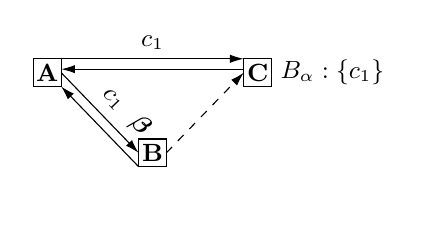
\begin{tikzpicture}[scale=1]
  
  \small
  
  \newcommand\X{190/5pt};
  \newcommand\Y{29pt};

  
  \draw[fill=white] (0*\X, 0*\Y) node{\textbf{A}} +(-5pt, -5pt) rectangle +(5pt, 5pt);
  % \draw (-5+0*\X, 0*\Y) node[left]{$E: \{a:2\}$};
  \draw[fill=white] (1*\X, -1*\Y) node{\textbf{B}} +(-5pt, -5pt) rectangle +(5pt, 5pt);
  \draw (5+ 1*\X, -5-1*\Y) node[below right]{\phantom{$B_\beta:\{b_1\}$}};
  \draw[fill=white] (2*\X,  0*\Y) node{\textbf{C}} +(-5pt, -5pt) rectangle +(5pt, 5pt);
  \draw (5+2*\X, 0*\Y) node[right]{$B_\alpha: \{c_1\}$};

  % \draw(2*\X, 5+0*\Y) node[above]{$\alpha$};
  % \draw (5+2*\X, 0*\Y) node[right]{$B_\alpha: \{c_1\}$};
  
  \draw[->](5+0*\X, 0*\Y) -- node[sloped,above]{~~~~$c_1$~~$\bm{\beta}$} (-5+1*\X, -1*\Y); %% A->B
  \draw[<-](5+0*\X, -5+0*\Y) -- (-5+1*\X, -5-1*\Y); %% A<-B
  
  \draw[->](5+0*\X, 5+0*\Y) -- node[above]{$c_1$} (-5+2*\X, 5+0*\Y); % A->C
  \draw[<-](5+0*\X,  1.25+ 0*\Y) -- (-5+2*\X,  1.25+ 0*\Y); % A<-C
  
  \draw[->,dashed](5+1*\X, -1*\Y) -- (-5+2*\X, 0*\Y); %% B<-C
  % \draw[->, dashed](5+1*\X, -5-1*\Y) -- (-5+2*\X, -5+0*\Y); %% B->C



\end{tikzpicture}%
      \caption{\label{fig:solveD}Process~A receives $\beta$ and routes it to
        Process~B.  Process~A receives $c_1$ and forwards it to both its
        neighbors.}
    \end{subfigure}
    ~
    \begin{subfigure}[t]{0.48\textwidth}
      \centering
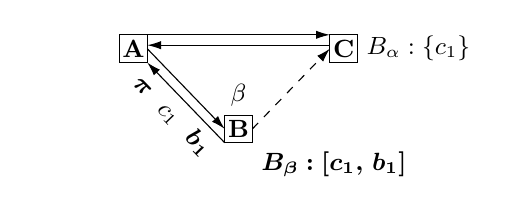
\begin{tikzpicture}[scale=1]
  
  \small
  
  \newcommand\X{190/5pt};
  \newcommand\Y{29pt};

  \draw (-1*\X, 0*\Y);
  \draw (3*\X, 0*\Y);
  
  \draw[fill=white] (0*\X, 0*\Y) node{\textbf{A}} +(-5pt, -5pt) rectangle +(5pt, 5pt);
  % \draw (-5+0*\X, 0*\Y) node[left]{$E: \{a:2\}$};
  \draw[fill=white] (1*\X, -1*\Y) node{\textbf{B}} +(-5pt, -5pt) rectangle +(5pt, 5pt);
  \draw (1*\X, 5-1*\Y) node[above]{$\beta$};
  \draw (5+ 1*\X, -5-1*\Y) node[below right]{$\bm{B_\beta: [c_1,\,b_1]}$};
  % \draw (1*\X, -5-1*\Y) node[below]{$E: \varnothing$\vphantom{$\{$}};
  \draw[fill=white] (2*\X,  0*\Y) node{\textbf{C}} +(-5pt, -5pt) rectangle +(5pt, 5pt);

  \draw (5+2*\X, 0*\Y) node[right]{$B_\alpha: \{c_1\}$};

  % \draw(2*\X, 5+0*\Y) node[above]{$\alpha$};
  % \draw (5+2*\X, 0*\Y) node[right]{$B_\alpha: \{c_1\}$};
  
  \draw[->](5+0*\X, 0*\Y) -- (-5+1*\X, -1*\Y); %% A->B
  \draw[<-](5+0*\X, -5+0*\Y) -- node[sloped, below]{$\bm{\pi}$~~$c_1$~~$\bm{b_1}$} (-5+1*\X, -5-1*\Y); %% A<-B
  
  \draw[->](5+0*\X, 5+0*\Y) -- (-5+2*\X, 5+0*\Y); % A->C
  \draw[<-](5+0*\X,  1.25+ 0*\Y) -- (-5+2*\X,  1.25+ 0*\Y); % A<-C
  
  \draw[->,dashed](5+1*\X, -1*\Y) -- (-5+2*\X, 0*\Y); %% B<-C
  % \draw[->, dashed](5+1*\X, -5-1*\Y) -- (-5+2*\X, -5+0*\Y); %% B->C



\end{tikzpicture}
%
      \caption{\label{fig:solveE}Process~C receives and discards
        $c_1$.  Process~B receives $\beta$ and replies $\pi$ to
        Process~C using Process~A as mediator.  Process~B receives
        $c_1$ and forwards it to its neighbor.  Process~B broadcasts
        $b_1$. It registers $c_1$ and $b_1$ in $B_\beta$.}
    \end{subfigure}    
    \begin{subfigure}[t]{0.48\textwidth}
      \centering
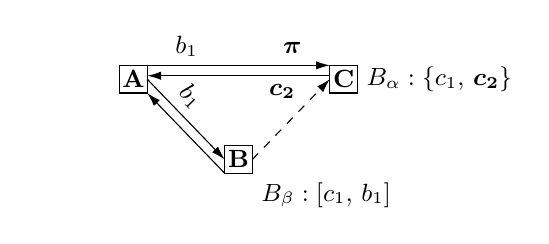
\begin{tikzpicture}[scale=1]
  
  \small
  
  \newcommand\X{190/5pt};
  \newcommand\Y{29pt};

  \draw (-1*\X, 0*\Y);
  \draw (3*\X, 0*\Y);
  
  \draw[fill=white] (0*\X, 0*\Y) node{\textbf{A}} +(-5pt, -5pt) rectangle +(5pt, 5pt);
  % \draw (-5+0*\X, 0*\Y) node[left]{$E: \{a:2\}$};
  \draw[fill=white] (1*\X, -1*\Y) node{\textbf{B}} +(-5pt, -5pt) rectangle +(5pt, 5pt);
  % \draw (1*\X, 5-1*\Y) node[above]{$\beta$};
  \draw (5+ 1*\X, -5-1*\Y) node[below right]{$B_\beta: [c_1,\,b_1]$};
  % \draw (1*\X, -5-1*\Y) node[below]{$E: \varnothing$\vphantom{$\{$}};
  \draw[fill=white] (2*\X,  0*\Y) node{\textbf{C}} +(-5pt, -5pt) rectangle +(5pt, 5pt);
  % \draw(2*\X, 5+0*\Y) node[above]{$\alpha$};
  \draw (5+2*\X, 0*\Y) node[right]{$B_\alpha: \{c_1,\, \bm{c_2}\}$};
  
  \draw[->](5+0*\X, 0*\Y) -- node[above, sloped]{$b_1$~~~~} (-5+1*\X, -1*\Y); %% A->B
  \draw[<-](5+0*\X, -5+0*\Y) -- (-5+1*\X, -5-1*\Y); %% A<-B
  
  \draw[->](5+0*\X, 5+0*\Y) -- node[above]{$b_1$~~~~~~~~~~$\bm{\pi}$} (-5+2*\X, 5+0*\Y); % A->C
  \draw[<-](5+0*\X,  1.25+ 0*\Y) -- (-5+2*\X,  1.25+ 0*\Y) node[below left]{$\bm{c_2}$~~~~}; % A<-C
  
  \draw[->,dashed](5+1*\X, -1*\Y) -- (-5+2*\X, 0*\Y); %% B<-C
  % \draw[->, dashed](5+1*\X, -5-1*\Y) -- (-5+2*\X, -5+0*\Y); %% B->C



\end{tikzpicture}
%
      \caption{\label{fig:solveF}Process~A receives $c_1$ and discards it.
        Process~A receives $\pi$ and routes it to Process~C. Process~A receives
        $b_1$ and forwards it to its neighbors. Process~C broadcasts $c_2$ and
        registers it in $B_\alpha$}
    \end{subfigure}
    ~
    \begin{subfigure}[t]{0.48\textwidth}
      \centering
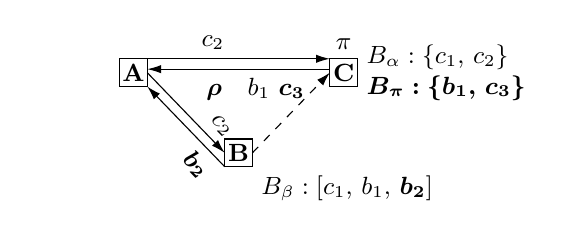
\begin{tikzpicture}[scale=1]
  
  \small
  
  \newcommand\X{190/5pt};
  \newcommand\Y{29pt};

  \draw (-1*\X, 0*\Y);
  \draw (3*\X, 0*\Y);
  
  \draw[fill=white] (0*\X, 0*\Y) node{\textbf{A}} +(-5pt, -5pt) rectangle +(5pt, 5pt);
  % \draw (-5+0*\X, 0*\Y) node[left]{$E: \{a:2\}$};
  \draw[fill=white] (1*\X, -1*\Y) node{\textbf{B}} +(-5pt, -5pt) rectangle +(5pt, 5pt);
  % \draw (1*\X, 5-1*\Y) node[above]{$\pi$};
  \draw (5+ 1*\X, -5-1*\Y) node[below right]{$B_\beta: [c_1,\,b_1,\,\bm{b_2} ]$};
  % \draw (1*\X, -5-1*\Y) node[below]{$E: \varnothing$\vphantom{$\{$}};
  \draw[fill=white] (2*\X,  0*\Y) node{\textbf{C}} +(-5pt, -5pt) rectangle +(5pt, 5pt);
  \draw(2*\X, 5+0*\Y) node[above]{$\pi$};
  \draw (5+2*\X, 0*\Y) node[right, align=left]{$B_\alpha: \{c_1,\, c_2\}$\\
  $\bm{B_\pi: \{ b_1,\, c_3 \}}$};
  
  \draw[->](5+0*\X, 0*\Y) -- node[sloped, above]{~~~~~~~ $c_2$} (-5+1*\X, -1*\Y); %% A->B
  \draw[<-](5+0*\X, -5+0*\Y) -- node[below, sloped]{~~~~~~~ $\bm{b_2}$} (-5+1*\X, -5-1*\Y); %% A<-B
  
  \draw[->](5+0*\X, 5+0*\Y) -- node[above]{$c_2$ ~~~~~~} (-5+2*\X, 5+0*\Y); % A->C
  \draw[<-](5+0*\X,  1.25+ 0*\Y) -- node[below]{~~~ $\bm{\rho}$ ~ $b_1$ $\bm{c_3}$} (-5+2*\X,  1.25+ 0*\Y); % A<-C
  
  \draw[->,dashed](5+1*\X, -1*\Y) -- (-5+2*\X, 0*\Y); %% B<-C
  % \draw[->, dashed](5+1*\X, -5-1*\Y) -- (-5+2*\X, -5+0*\Y); %% B->C



\end{tikzpicture}
%
      \caption{\label{fig:solveG}Process~A receives $c_2$ and forwards it to
        its neighbors.  Process~B broadcasts $b_2$ and registers it in
        $B_\beta$. Process~C receives $\pi$ and replies $\rho$ to Process~B
        using Process~A as mediator. Then it receives and forwards $b_1$. Then
        it broadcasts $c_3$. It registers $b_1$ and $c_3$ in $B_\pi$.}
    \end{subfigure}
    \begin{subfigure}[t]{0.48\textwidth}
      \centering
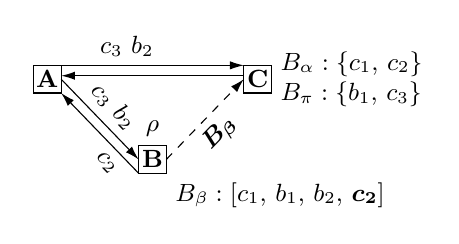
\begin{tikzpicture}[scale=1]
  
  \small
  
  \newcommand\X{190/5pt};
  \newcommand\Y{29pt};

  
  \draw[fill=white] (0*\X, 0*\Y) node{\textbf{A}} +(-5pt, -5pt) rectangle +(5pt, 5pt);
  % \draw (-5+0*\X, 0*\Y) node[left]{$E: \{a:2\}$};
  \draw[fill=white] (1*\X, -1*\Y) node{\textbf{B}} +(-5pt, -5pt) rectangle +(5pt, 5pt);
  \draw (1*\X, 5-1*\Y) node[above]{$\rho$};
  \draw (5+ 1*\X, -5-1*\Y) node[below right]{$B_\beta: [c_1,\,b_1,\,b_2,\,\bm{c_2}]$};
  % \draw (1*\X, -5-1*\Y) node[below]{$E: \varnothing$\vphantom{$\{$}};
  \draw[fill=white] (2*\X,  0*\Y) node{\textbf{C}} +(-5pt, -5pt) rectangle +(5pt, 5pt);
  % \draw(2*\X, 5+0*\Y) node[above]{$\pi$};
  \draw (5+2*\X, 0*\Y) node[right, align=left]{$B_\alpha: \{c_1,\, c_2\}$\\$B_\pi: \{ b_1,\, c_3 \}$};
  
  \draw[->](5+0*\X, 0*\Y) -- node[sloped, above] {$c_3$ $b_2$} (-5+1*\X, -1*\Y); %% A->B
  \draw[<-](5+0*\X, -5+0*\Y) -- node[sloped, below]{~~~~~ $c_2$} (-5+1*\X, -5-1*\Y); %% A<-B
  
  \draw[->](5+0*\X, 5+0*\Y) -- node[above]{$c_3$ $b_2$ ~~~~~~} (-5+2*\X, 5+0*\Y); % A->C
  \draw[<-](5+0*\X,  1.25+ 0*\Y) -- (-5+2*\X,  1.25+ 0*\Y); % A<-C
  
  \draw[->,dashed](5+1*\X, -1*\Y) -- node[below, sloped]{$\bm{B_\beta}$} (-5+2*\X, 0*\Y); %% B<-C
  % \draw[->, dashed](5+1*\X, -5-1*\Y) -- (-5+2*\X, -5+0*\Y); %% B->C



\end{tikzpicture}
%
      \caption{\label{fig:solveH}Process~A receives and discards $b_1$.
        Process~A receives and routes $\rho$ to Process~B.  Process~A receives
        and forwards $b_2$ then $c_3$. Process~B receives, forwards, and
        registers $c_2$. Then Process~B receives $\rho$ and sends $B_\beta$ to
        Process~C using the new link.}
    \end{subfigure}
    ~
    \begin{subfigure}[t]{0.48\textwidth}
      \centering
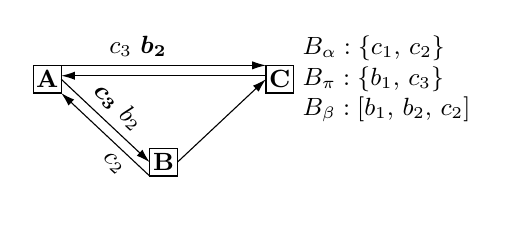
\begin{tikzpicture}[scale=1]
  
  \small
  
  \newcommand\X{210/5pt};
  \newcommand\Y{30pt};

  
  \draw[fill=white] (0*\X, 0*\Y) node{\textbf{A}} +(-5pt, -5pt) rectangle +(5pt, 5pt);
  % \draw (-5+0*\X, 0*\Y) node[left]{$E: \{a:2\}$};
  \draw[fill=white] (1*\X, -1*\Y) node{\textbf{B}} +(-5pt, -5pt) rectangle +(5pt, 5pt);
  % \draw (1*\X, 5-1*\Y) node[above]{$\rho$};
  \draw (5+ 1*\X, -5-1*\Y) node[below right]{\phantom{$B_\beta: [b_1,\,b_2,\,c_2]$}};
  % \draw (1*\X, -5-1*\Y) node[below]{$E: \varnothing$\vphantom{$\{$}};
  \draw[fill=white] (2*\X,  0*\Y) node{\textbf{C}} +(-5pt, -5pt) rectangle +(5pt, 5pt);
  % \draw(2*\X, 5+0*\Y) node[above]{$\pi$};
  \draw (5+2*\X, 0*\Y) node[right, align=left]{$B_\alpha: \{c_1,\, c_2\}$\\$B_\pi: \{ b_1,\, c_3 \}$\\$B_\beta: [b_1,\,b_2,\,c_2]$};
  
  \draw[->](5+0*\X, 0*\Y) -- node[sloped, above] {$\bm{c_3}$ $b_2$} (-5+1*\X, -1*\Y); %% A->B
  \draw[<-](5+0*\X, -5+0*\Y) -- node[sloped, below]{~~~~~ $c_2$} (-5+1*\X, -5-1*\Y); %% A<-B
  
  \draw[->](5+0*\X, 5+0*\Y) -- node[above]{$c_3$ $\bm{b_2}$ ~~~~~~} (-5+2*\X, 5+0*\Y); % A->C
  \draw[<-](5+0*\X,  1.25+ 0*\Y) -- (-5+2*\X,  1.25+ 0*\Y); % A<-C
  
  \draw[->](5+1*\X, -1*\Y) -- (-5+2*\X, 0*\Y); %% B<-C
  % \draw[->, dashed](5+1*\X, -5-1*\Y) -- (-5+2*\X, -5+0*\Y); %% B->C
\end{tikzpicture}%
      \caption{\label{fig:solveI}Once Process~A sent $B_\beta$, the new link is
        safe.  Process~C receives $B_\beta$. Process~C does not deliver $c_1$, $b_1$
        and $c_2$, for it already delivered them. Process~C delivers $b_2$ and
        expects another copy from Process~A, for it constitutes a new message.
        Process~C expects to eventually receive $c_3$ from Process~B.}
    \end{subfigure}
    \begin{subfigure}[t]{0.99\textwidth}
      \centering
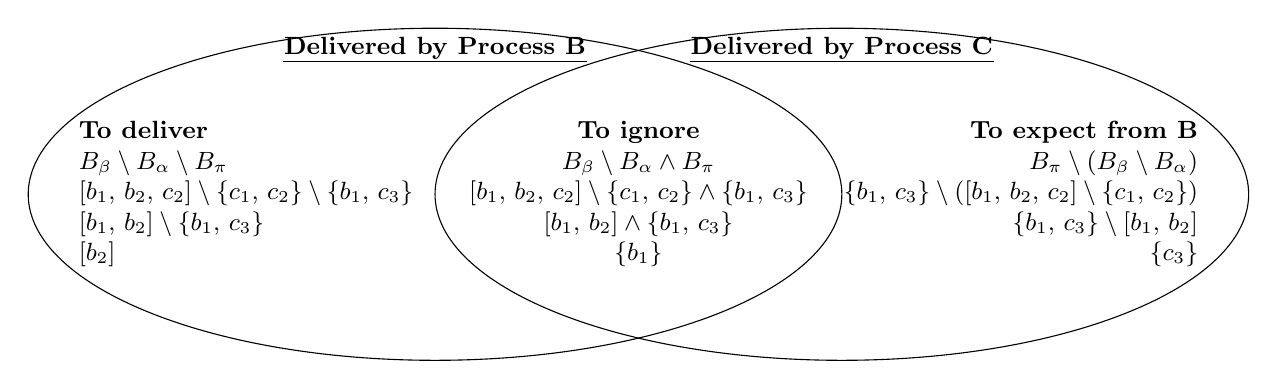
\begin{tikzpicture}[scale=1]

  \small
  
  \newcommand\X{210/5pt};
  \newcommand\Y{30pt};
  
  \newcommand\RADX{3.5};
  \newcommand\RADY{2};

  \newcommand\OFFX{15pt};

  \draw (0*\X, 0pt) circle [x radius=\RADX*\X, y radius = \RADY*\Y];
  \draw (0*\X, \RADY*\Y) node[below]{\textbf{\uline{Delivered by Process~B}}};

  \draw (\OFFX-\RADX*\X, 0pt) node[right, align=left] {
    \textbf{To deliver}\\%\tiny
    $B_\beta \setminus B_\alpha \setminus B_\pi$\\%\tiny
    $[b_1,\,b_2,\,c_2]\setminus\{c_1,\,c_2\}\setminus\{b_1,\,c_3\}$\\%\tiny
    $[b_1,\,b_2] \setminus \{b_1,\,c_3\}$\\%\tiny
    $[b_2]$
  };
  \draw (-\OFFX+2*\RADX*\X, 0pt) node[left, align=right] {
    \textbf{To expect from B}\\%\tiny
    $B_\pi \setminus (B_\beta \setminus B_\alpha)$\\%\tiny
    $\{b_1,\,c_3\} \setminus ([b_1,\,b_2,\,c_2] \setminus\{c_1,\,c_2\})$\\%\tiny
    $\{b_1,\,c_3\} \setminus [b_1,\,b_2]$\\%\tiny
    $\{c_3\}$
  };
  \draw (0.5*\RADX*\X, 0pt) node[align=center] {
    \textbf{To ignore}\\%\tiny
    $B_\beta \setminus B_\alpha \wedge B_\pi$\\%\tiny
    $[b_1,\,b_2,\,c_2] \setminus \{c_1,\,c_2\} \wedge \{ b_1,\,c_3\}$\\%\tiny
    $[b_1,\,b_2] \wedge \{ b_1, \, c_3 \}$\\%\tiny
    $\{ b_1 \}$
  };
  \draw (\RADX*\X, 0pt) circle [x radius=\RADX*\X, y radius = \RADY*\Y];
  \draw (\RADX*\X, \RADY*\Y) node[below]{\textbf{\uline{Delivered by Process~C}}};
\end{tikzpicture}
%
      \caption{\label{fig:solveJ}Process~C categorizes each message of $B_\beta$
        and $B_\pi$ to maintain and initialize safe link memory.}
    \end{subfigure}
    \caption{\label{fig:solve}Using buffers and control messages, \RPCBROADCAST 
      provides reliable causal broadcast.}
  \end{center}
\end{figure}

\begin{algorithm}[h]
  \SetKwProg{Function}{function}{}{}
\SetKwProg{Upon}{upon}{}{}
\SetKwProg{Initially}{INITIALLY:}{}{}
\SetKwProg{Safety}{SAFETY:}{}{}
\SetKwProg{Dissemination}{DISSEMINATION:}{}{}

\small

\DontPrintSemicolon
\LinesNumbered

%\begin{multicols}{2}
\Initially {} {
  $Q_o$ \tcp*{Set of processes, $p$'s outview}
  $Q_i$ \tcp*{Set of processes, $p$'s inview}
  \BlankLine  
  $B \leftarrow \varnothing$ \tcp*{link $\rightarrow$ buffered messages}
  \BlankLine  
  $S \leftarrow \varnothing$ \tcp*{Map of buffers $Q_i : M^* \times M^* \times bool$}
}

\BlankLine

\Safety{}{
  
  \Upon{$\textup{open}_o(q)$} {
    $Q_o \leftarrow Q_o \setminus q$ \;
    $\textup{sendAlpha}(p,\,q)$ \label{line:sendalpha} \tcp*{$\alpha$}
  }
  
  \Upon{$\textup{open}_i(q)$} {
    $Q_i \leftarrow Q_i \setminus q$ \;
  }

  \BlankLine
  
  \Upon{$\textup{receiveAlpha}(from,\,to)$ \tcp*[f]{$to=p$}} {
    $S[from] \leftarrow \langle \varnothing,\, \varnothing,\, false \rangle$ 
    \tcp*{$B_\alpha$}
    $\textup{sendBeta}(from,\,to)$ \label{line:sendbeta} \tcp*{$\beta$}
  }

  \BlankLine

  \Upon{$\textup{receiveBeta}(from,\,to)$ \tcp*[f]{$from=p$}} {
    $B[to] \leftarrow \varnothing$ \tcp*{$B_\beta$}
    $\textup{sendPing}(from,\, to)$ \label{line:sendpi} \tcp*{$\pi$}
  }
  
  \BlankLine

  \Upon{$\textup{receivePing}(from,\,to)$ \tcp*[f]{$to=p$}} {
    \textbf{let} $\langle B_\alpha ,\, B_\pi ,\, \_ \rangle \leftarrow S[from]$ \;
    $S[from] \leftarrow \langle B_\alpha,\, B_\pi,\, true \rangle$ \tcp*{$B_\pi$}
    $\textup{sendPong}(from,\, to)$ \label{line:sendrho} \tcp*{$\rho$}
  }

  \BlankLine

  \Upon{$\textup{receivePong}(from,\,to)$ \tcp*[f]{$from=p$}} {
    $\textup{sendBuffer}(from,\,to,\, B[to])$ \;
    $B \leftarrow B \setminus to$ \;
    $Q_o \leftarrow Q_o \cup to$
  }

  \BlankLine

  \Upon{$\textup{receiveBuffer}(from,\, to,\, B_\beta)$} {
    \textbf{let} $\langle B_\alpha,\, B_\pi,\, \_ \rangle \leftarrow S[from]$ \;
%    \textbf{let} $potential \leftarrow buf \setminus B_\alpha$ \;
    \ForEach {$m \in B_\beta\setminus B_\alpha \setminus B_\pi$ }
    {$\textup{receive}(m,\,from)$ \tcp*[f]{to deliver}}
    $D[from] \leftarrow B_\pi \setminus (B_\beta\setminus B_\alpha)$ \tcp*{to expect}
    $Q_i \leftarrow Q_i \cup from$ 
  }
  
  \BlankLine

  \Upon{$\textup{close}_o(q)$} {
    $B \leftarrow B \setminus q$
  }
  \Upon{$\textup{close}_i(q)$} {
    $S \leftarrow S \setminus q$
  }

  
}

\BlankLine

\Dissemination{}{
  
  \Function{$\RPCBROADCAST(m)$} { %\tcp*[f]{$b_p(m)$}} {
    $\textup{buffering}(m)$ \;
    $\textup{R-broadcast}(m)$
  }

  \BlankLine
  
  \Upon{$\textup{R-deliver}(m)$} {
    $\textup{buffering}(m)$ \;
    $\textup{RPC-deliver}(m)$
  }

  \BlankLine

  \Function{$\textup{buffering}(m)$}{ 
    \lForEach {$q \in B$} {$B[q] \leftarrow B[q] \cup m$}
    \ForEach {$q \in S$} {
      \textbf{let} $\langle B_\alpha,\, B_\pi,\, received_\pi \rangle \leftarrow S[q]$ \;
      \lIf {$received_\pi$} {$B_\pi \leftarrow B_\pi \cup m$}
      \lElse {$B_\alpha \leftarrow B_\alpha \cup m$} 
    }
  }
}
%\end{multicols}

%%% Local Variables:
%%% mode: latex
%%% TeX-master: "../paper"
%%% End:

  \caption{\label{algo:rpcbroadcast}\RPCBROADCAST at Process $p$.}
\end{algorithm}


Algorithm~\ref{algo:rpcbroadcast} shows the instructions of \RPCBROADCAST. 
Figure~\ref{fig:solve} illustrates its operation in a scenario involving 3
processes. In this example, Process~B adds a link to Process~C. Process~B
disables the new link for causal broadcast until it is safe and guaranteed that
Process~C correctly initialized its memory.

\noindent Process~B sends a first control message $\alpha$ to Process~B using
safe links (see Line~\ref{line:sendalpha} and Figure~\ref{fig:solveA}).

\noindent After being routed to Process~C by intermediary processes (see
Figure~\ref{fig:solveB}), $\alpha$ reaches Process~C (see
Figure~\ref{fig:solveC}).  Process~C starts to register messages it delivers in
a buffer $B_\alpha$.  Process~C acknowledges the receipt of $\alpha$ by sending
a second control message $\beta$ to Process~B using safe links (see
Line~\ref{line:sendbeta}). In Figure~\ref{fig:solveC}, Process~C broadcasts
$c_1$ and registers it in $B_\alpha$.

\noindent After being routed to Process~B (see Figure~\ref{fig:solveD}), $\beta$
reaches Process~B. Process~B starts to register messages it delivers in a buffer
$B_\beta$. Process~B sends a third control message $\pi$ to Process~C using safe
links (see Line~\ref{line:sendpi}). In Figure~\ref{fig:solveE}, Process~B delivers
$c_1$ then broadcasts $b_1$. It registers them in $B_\beta$. In Figure~\ref{fig:solveF},
Process~C broadcasts $c_2$ and registers it in $B_\alpha$.

\noindent After being routed to Process~C by intermediary processes (see
Figure~\ref{fig:solveF}), $\pi$ reaches Process~C. Process~C ends its first
buffer $B_\alpha$.  Process~C starts to register messages it delivers in
$B_\pi$.  Process~C sends a fourth and last control message $\rho$ to Process~B
using safe links (see Line~\ref{line:sendrho}). In Figure~\ref{fig:solveG}
Process~C delivers $b_1$, broadcasts $c_3$, and registers them in $B_\pi$. In
the meantime, Process~B broadcasts $b_2$ and registers it in $B_\beta$.

\noindent After being routed to Process~B, $\rho$ reaches Process~B (see
Figure~\ref{fig:solveH}).  Process~B stops buffering and sends its buffer of
messages $B_\beta$ using the new link $s_{BC}(B_\beta)$ (see
Line~\ref{line:sendbuffer}). In Figure~\ref{fig:solveI}, this buffer contains
$b_1$, $b_2$, and $c_2$. The new link is safe. Process~B starts to use this link
normally for causal broadcast using Algorithm~\ref{algo:reliablebroadcast}.

\noindent Once Process~C receives the buffer, it ends its buffer $B_\pi$ (see
Figure~\ref{fig:solveI}). Using $B_\alpha$, and $B_\pi$, Process~C identifies
among messages from $B_\beta$ the array of messages to deliver (see
Line~\ref{line:todeliver}). In Figure~\ref{fig:solveJ}, this array only includes
$b_2$.  Using $B_\alpha$, and $B_\pi$, Process~C also identifies the set of
messages to ignore which is the rest of the buffer. In Figure~\ref{fig:solveJ},
this set includes $c_1$, $b_1$ and $c_2$. Finally, Process~C identifies among its own
delivered messages the messages to expect from Process~B (see
Line~\ref{line:toexpect}). In Figure~\ref{fig:solveJ}, this set includes $c_3$.
This set constitutes the memory of the new safe link.  Afterwards, messages
received by this new link are processed normally.


\RPCBROADCAST builds safe link memory using control messages that follow causal
order. Link memory forbids multiple delivery and implies non-monotonic space
complexity. In the next section, we analyze the complexity of our causal
broadcast implementation.

\subsection{Complexity}
\label{subsec:complexity}

In this section, we analyze the complexity of \RPCBROADCAST in terms of
broadcast message overhead, delivery execution time, local space consumption,
and number of control messages.

\noindent The \textbf{broadcast message overhead} is constant $O(1)$. Messages
must travel using FIFO links.

\noindent The \textbf{delivery execution time}, i.e., the time complexity of the
receipt function is $O(Q_i)$. It checks and update control information
associated to each link in the in-view.

\noindent The \textbf{local space consumption} depends on the size of buffers
and the size of the in-view. Each link in the in-view has its buffer of control
information about messages. A message appears in the structure after its first
receipt and disappears at its last receipt. So the local space complexity is
$O(Q_i.M)$ where $M$ is the number of messages already delivered that should be
received again from at least one process in $Q_i$. A process stores the control
information of a message during at most $D$ time where $D$ is the diameter of
the system. The local space consumption depends on the system (e.g. ring or tree
topologies do not consume any space) and its usage (e.g. when no process
broadcasts any message, processes do not consume any space).
% Similarly to \PCBROADCAST, the size of buffers may increase unbounded when
% intermediate processes are faulty. Control messages never reach their
% destination. \PCBROADCAST handles such crashes using a timeout and retry
% policy. Such strategy fits \RPCBROADCAST as well. Both involved processes can
% halt and retry the safety check of the new link. Either the origin process does
% not send its buffer $B_\beta$, or the destination process does not accept
% incoming messages. 

\noindent The overhead in terms of \textbf{number of control messages} per added
link in an out-view varies from $6$ to $4P^2$ depending on the overlay network;
$P$ being the number of processes in the system. It achieves $6$ messages when
Process~A adds Process~B using Process~C as mediator, and Process~B has
Process~A in its out-view.  It achieves $8$ control messages when peer-sampling
protocols build out-views using neighbor-to-neighbor
interactions~\cite{jelasity2007gossip,nedelec2017adaptive}. It achieves
$O(\log(P))$ control messages when peer-sampling protocols allows processes to
route their messages~\cite{jelasity2009tman,stoica2001chord}.  It achieves
$O(4P^2)$ control messages when Process~A adds Process~B without knowledge of
any route. Process~A and Process~B fall back to reliable broadcast instead of
routing to disseminate control messages.

This complexity analysis shows that \RPCBROADCAST proposes an original tradeoff
in terms of complexity. In systems allowing a form of routing, it constitutes an
advantageous tradeoff that depends on the actual system instead of past
deliveries. The next section describes an experiment highlighting the effects of
the system settings on the space consumed by processes.

%%% Local Variables:
%%% mode: latex
%%% TeX-master: "../paper"
%%% End:


\section{Experimentation}
\label{sec:experimentation}

\RPCBROADCAST proposes an original tradeoff in terms of complexity. Among other,
it removes the last monotonic and linear upper bound that remained on space
complexity. In this section, we evaluate the impact of the actual system on the
space consumed and traffic generated by processes. The experiments run on the
\PEERSIM simulator~\cite{montresor2009peersim} that allows to build large and
dynamic systems. Our implementation is available on the Github platform at
\url{http://github.com/chat-wane/peersim-prcbroadcast}. \\


% \begin{figure}
%   \begin{center}
%   
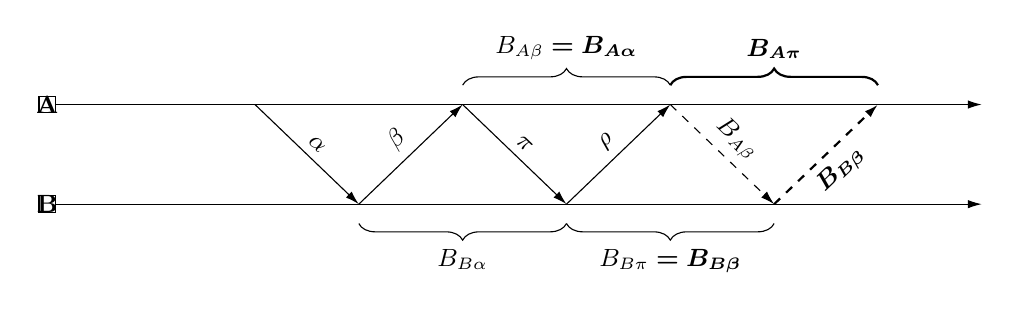
\begin{tikzpicture}[scale=0.6]

  \small
  
  \newcommand\X{1.45*\columnwidth/8pt};
  \newcommand\YA{0pt};
  \newcommand\YB{-60pt};


  \draw[->](0*\X, \YA) -- (9*\X, \YA);
  \draw[->](0*\X, \YB) -- (9*\X, \YB);
  
  \draw[fill=white] (0*\X, \YA) node{\textbf{\textup{A}}}
  +(-5pt, -5pt) rectangle +(5pt, 5pt);
  \draw[fill=white] (0*\X, \YB)  node{\textbf{\textup{B}}}
  +(-5pt, -5pt) rectangle +(5pt, 5pt);

  % \draw ( 1*\X, \YA ) node[above]{$\mathcal{A}$};
  % \draw ( 1*\X, \YB ) node[below]{$\mathcal{B}$};

  \draw[->] ( 2*\X, \YA ) -- node[sloped, above]{$\alpha$} (3*\X, \YB);
  % node[below left]{$\mathcal{A}$};

  \draw[decorate,decoration={brace,amplitude=6pt,mirror,raise=4pt}] (3*\X,
  -5+\YB) -- node[anchor=north, yshift=-10pt]{$B_{B\alpha}$}
  (5*\X, -5+\YB);

  % \draw ( 3*\X, \YA ) node[above]{$\mathcal{C}$};

  \draw[->] ( 3*\X, \YB ) -- node[sloped, above]{$\beta$} (4*\X, \YA);
  % node[above left]{$\mathcal{B}$};

  \draw[decorate,decoration={brace,amplitude=6pt,raise=4pt}] (4*\X,
  5+\YA) -- node[anchor=south, yshift=10pt]{$B_{A\beta} \bm{= B_{A\alpha}}$}
  (6*\X, 5+\YA);

  \draw[decorate,thick,decoration={brace,amplitude=6pt,raise=4pt}] (6*\X,
  5+\YA) -- node[anchor=south, yshift=10pt]{$\bm{B_{A\pi}}$}
  (8*\X, 5+\YA);
  
  
  % \draw ( 4*\X, \YB ) node[below]{$\mathcal{D}$};

  \draw[->] ( 4*\X, \YA ) -- node[sloped, above]{$\pi$} (5*\X, \YB);
  % node[below left]{$\mathcal{C}$};

  \draw[decorate,decoration={brace,amplitude=6pt,mirror,raise=4pt}] (5*\X,
  -5+\YB) -- node[anchor=north, yshift=-10pt]{$B_{B\pi} \bm{= B_{B\beta}}$}
  (7*\X, -5+\YB);


  % \draw ( 5*\X, \YA ) node[above]{$\mathcal{E}$};

  \draw[->] ( 5*\X, \YB ) -- node[sloped, above]{$\rho$} (6*\X, \YA);
  % node[above left]{$\mathcal{D}$};
  
  % \draw (6*\X, \YB) node[below]{$\mathcal{F}$};

  \draw[->, dashed] ( 6*\X, \YA ) -- node[sloped, above]{$B_{A\beta}$} (7*\X, \YB);

  \draw[->, dashed, thick] ( 7*\X, \YB ) --
  node[sloped, below]{$\bm{B_{B\beta}}$} (8*\X, \YA);

%  node[below left]{$\mathcal{E}$};


\end{tikzpicture}

%%% Local Variables:
%%% mode: latex
%%% TeX-master: "../paper"
%%% End:

%   \caption{\label{fig:bibroadcast}\RPCBROADCAST ensures the safety of bidirectional links
%     at marginal cost. Process~A maintains an additional buffer. Process~B transmits its
%     second buffer.}
%   \end{center}
% \end{figure}

% When links are bidirectional, \RPCBROADCAST must ensure their safety
% in both directions. Instead of performing twice \RPCBROADCAST's
% operation, we extend its behavior to handle bidirectional safety at
% once. Some control messages serve two purposes. For instance, control
% messages $\beta$ are also control messages $\alpha$. Some buffers have
% two purposes. For instance, the buffer $B_\beta$ of the process adding
% a link is also a buffer $B_\alpha$.  Figure~\ref{fig:bibroadcast}
% depicts the small change in the operation of \RPCBROADCAST. It ensures
% safety of bidirectional links at marginal cost compared to its
% unidirectional version. The buffer $B_\beta$ of Process~A becomes its
% buffer $B_\alpha$. The buffer $B_\pi$ of Process~B becomes a buffer
% $B_\beta$ that will be sent using the new link upon receipt of the
% buffer of Process~A. Between the sending of its buffer and the receipt
% of the buffer of Process~B, Process~A maintains an additional buffer
% $B_\pi$. \TODO{Maybe move this in proposal?}


\noindent \textbf{Objective:} To confirm that local space complexity
depends on in-views and message receipts.

\noindent \textbf{Description:} We measure the average size of buffers and
arrays of expected messages. This constitutes the average local space overhead
consumed by \RPCBROADCAST to detect and forbid multiple delivery in dynamic
systems.\\
Runs involve 3 overlay networks comprising 100, 1k, and 10k
processes. \SPRAY~\cite{nedelec2017adaptive} builds an highly dynamic overlay
networks that allows balancing the traffic generated by broadcasting among
processes. Each process maintains a neighborhood logarithmically scaling with
the number of processes in the system. Each process of the 100-processes system
has a neighborhood of $\approx 10$ neighbors. Each process of the 1k-processes
system has a neighborhood of $\approx 13.5$ neighbors. Each process of the
10k-processes system has a neighborhood of $\approx 15$ neighbors. Each process
dynamically re-configure their neighborhood every minutes by exchanging safe
links with a chosen neighbor: it gives half of its safe links to the chosen
neighbor; the latter gives half of its safe links to the former as well. Each
exchange leads to link memory initialization and safety checks of the new links,
and removal of given links.\\ Links are bidirectional, their safety must be
checked in both directions but the overhead remains minor. Links have
transmission delay, i.e., the time between the sending of a message and its
receipt is not null. The experiments start with $1ms$ delay. At $15min$ the
delay starts to increase. At ~$17min$ links reach $300ms$ delay. At $40min$
links reach $2.5s$ delay and it stops increasing.\\
From $2min$ to $50min$, every second, 10 processes chosen uniformly at random
among all processes broadcast a message.

\begin{figure}
  \begin{center}
    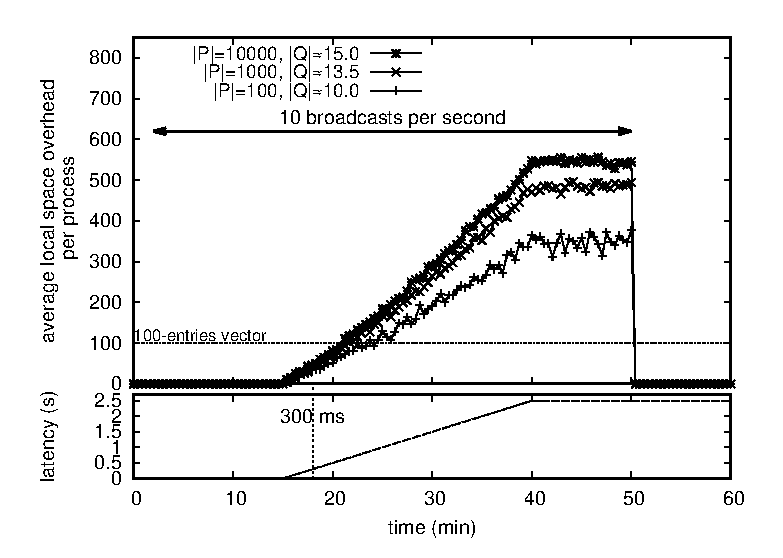
\includegraphics[width=0.8\columnwidth]{./img/overhead.eps}
    \caption{\label{fig:overhead}Local space overhead over time consumed by
      \RPCBROADCAST to ensure causal order and forbid double delivery in dynamic
      systems with varying latency.}
  \end{center}
\end{figure}

\noindent \textbf{Results:} Figure~\ref{fig:overhead} shows the result of this
experiment. The x-axis denotes the time in minute. The top part of the figure
shows local space overhead while the bottom part of the figure shows the
evolution of transmission delays. 

\begin{itemize}
\item Figure~\ref{fig:overhead} confirms that the local space consumption
  depends on the in-view size. Systems with larger in-views consume more
  space. Each new delivered message adds control information on each link of the
  in-view (see Algorithm~\ref{algo:reliablebroadcast}).
\item Figure~\ref{fig:overhead} confirms that the local space consumption
  depends on network condition. The overhead increases as the latency
  increases. Latency increases the time between the first and the last receipt
  of each message. Processes store messages longer until they can be safely
  removed. 
\item Figure~\ref{fig:overhead} confirms that the local space consumption
  depends on broadcast messages. When processes stops broadcasting, the space
  consumed at each process drops to 0. Each process eventually receive each
  message and safely remove the corresponding entry.
\item Figure~\ref{fig:overhead} shows that at a rate of 10 broadcasts per second
  and when latency stays under a realistic bound ($300ms$), the overhead is
  lower than vector-based approaches. Whatever system conditions, it would
  require a vector of 100, 1k entries, 10k entries to forbid multiple delivery
  in the 100-processes systems, 1k-processes system, 10k-processes system
  respectively.
\end{itemize}

\noindent \RPCBROADCAST provides a tradeoff where space complexity is
non-monotonic and actually depends on the system and its current usage; instead
of past usage using vectors of logical clocks. This result means that it
constitutes an advantageous tradeoff in
\begin{inparaenum}[(i)]
\item dynamic systems
\item comprising up to millions of processes
\item that could broadcast at any time.
\end{inparaenum} \\

\noindent \textbf{Objective:} To confirm that the generated traffic overhead
depends on the dynamicity of the system.

\noindent \textbf{Description:} We measure the average number of control
messages received by each process during a second. This includes the routing of
messages. The setup is identical to that of prior experiment.

\begin{figure}
  \begin{center}
    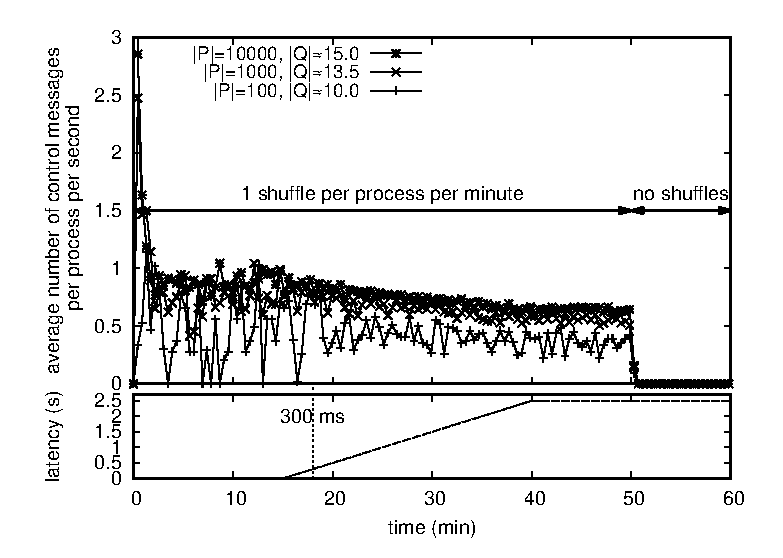
\includegraphics[width=0.8\columnwidth]{./img/controlmessages.eps}
    \caption{\label{fig:controlmessages}Traffic overhead generated by
      \RPCBROADCAST.  Average number of control messages received -- including
      forwarding -- per process for each second.}
  \end{center}
\end{figure}

\noindent \textbf{Results:} Figure~\ref{fig:controlmessages} shows the result of
this experiment. The top part of the figure shows traffic overhead generated by
\RPCBROADCAST while the bottom part of the figure shows the evolution of
transmission delays.

\begin{itemize}
\item Figure~\ref{fig:controlmessages} shows that the number of control messages
  received by processes depends on the dynamicity of the system. The more
  dynamic the higher the traffic overhead. At the beginning of the experiment,
  processes join the system and a high number of links must be established at
  once, hence the high number of control messages. Then processes shuffle their
  out-view during 50 minutes. The number of links to add and remove is roughly
  constant over time, hence the stabilization in number of control
  messages. Finally, processes stop shuffling at $50min$. Processes do not
  receive additional control messages.
\item Figure~\ref{fig:controlmessages} confirms our traffic overhead complexity
  analysis. For instance, in the 10k-processes system, views comprises 15
  processes which belong half from the out-view and half from the in-view.  Each
  process shuffles every minutes. Each shuffle adds and removes 7.5 links (twice
  half of the out-view size). Since the peer-sampling protocol establishes links
  using neighbor-to-neighbors interactions, it allows a form of routing where
  only 8 control messages are required to initialize a new link.
  $|exchanged\_links|*|control\_messages|/60 \approx 7.5*8/60 \approx 1$ control
  message per second.
\item Figure~\ref{fig:controlmessages} shows that latency decreases and smooth
  the number of control messages. The peer-sampling protocol only shuffles links
  already safe and the memory of which is initialized. Since increasing latency
  increases the initialization time of links, processes exchange less links at
  each shuffle. The generated traffic decreases accordingly. Latency also
  spreads control messages over time, hence the smoothing in measurements.
\end{itemize}

Overall, this section empirically confirms that the space complexity of
\RPCBROADCAST is non-monotonic and depends on the system and its
usage. Section~\ref{subsec:complexity} states that the space complexity is
$O(Q_i.M)$ where $Q_i$ is the size of the in-view built by peer-sampling
protocols, and $M$ is the number of messages that have been delivered but that
will be received again. This experiment confirms that the space consumed by each
process increases and decreases over time. In dynamic settings, this comes at
the cost of control messages to initialize memory link. This section shows that
this number remains small even in highly dynamic systems when peer-sampling
protocols allow a form of routing.  In this experiment, the underlying
peer-sampling protocol builds random graph topologies that have numerous
desirable properties such as crash resilience, or load
balancing~\cite{jelasity2007gossip}. This is ideal for systems where numerous
processes join and leave continuously. However, it is worth noting that it
remains in the hands of developers to choose the best peer-sampling protocol for
their system.


%Using \RPCBROADCAST, processes pay at the height of their current use instead of
%their past use.
The next section reviews state-of-the-art approaches designed to forbid multiple
delivery.




%%% Local Variables:
%%% mode: latex
%%% TeX-master: "../paper"
%%% End:


\section{Related work}
\label{sec:relatedwork}

Causal broadcast protocols rely on reliable
broadcast~\cite{hadzilacos1994modular}. Uniform reliable broadcast must ensure
that
\begin{inparaenum}[(i)]
\item all processes receive broadcast messages and
\item each process delivers each broadcast message once despite multiple
  receipts.
\end{inparaenum} This section reviews state-of-the-art from probabilistic
dissemination approaches to deterministic ones; from physical clock techniques
to vector-based approaches;

In large and dynamic systems comprising from hundreds to millions of processes,
gossiping constitutes the mean to disseminate
messages. \textbf{Non-deterministic} gossip-based
approaches~\cite{birman1999bimodal,demers1987epidemic} guarantee that each
process receives each broadcast message with high probability. Processes must be
able to identify and retrieve missing messages by themselves. In this paper, we
rely on \textbf{deterministic} gossip-based
approaches~\cite{nedelec2017adaptive} where peer-sampling protocols build
connected graph topology. Using all provided reliable links for broadcast
ensures that each process eventually receives each message.

Despite possible multiple receipts, processes must deliver messages at most
once. Approaches based on \textbf{dissemination
  pattern~\cite{bravo2017saturn,raynal2013distributed}} build topologies such as
tree or ring. Each process receives each message once, hence delivers it once,
without saving any control information. However, they stay confined to systems
where failures are uncommon. \RPCBROADCAST does not assume any specific
topology. It remains in the hand of developers to choose the best peer-sampling
protocol for their requirement and resources.

When multiple receipts can occur, each process maintains a local structure to
detect and discard copies of broadcast messages. Using \textbf{physical clocks
  (\REF)} allows removing control information over time. Control information is
considered obsolete above an age threshold. The structure is
non-monotonic. However, defining the age threshold is error prone. Set too small
and processes may suffer multiple delivery with cascading effects as in
Figure~\ref{fig:memorylinkfailsD}. \RPCBROADCAST maintains a non-monotonic
structure but makes sure that removed control information is truly obsolete.

Using \textbf{logical clocks}~\cite{malkhi2007concise,mukund2014optimized}
allows to discard all copies of broadcast messages. However, each process
maintains a vector with one entry per process that ever broadcast a message.
Processes cannot reclaim entries, for it would require running an overcostly
distributed garbage collection that is equivalent to a distributed consensus. As
consequence, the vector size increases linearly and monotonically. Vector-based
approaches do not scale in large and dynamic systems where any process can
broadcast a message at any time~\cite{nedelec2016crate}. \RPCBROADCAST's core
uses logical clocks too. Instead of encoding the global state of the system in a
vector, it only maintains its receipt state with its direct
neighborhood. Neighborhood being far smaller than the full system membership,
\RPCBROADCAST scales in large and dynamic systems. \\
However, vector clocks allow each process to perform anti-entropy with any other
process at any time. The former identifies its missing messages compared to the
latter.  The latter sends them to keep consistent states. This is useful when
applications can go offline~\cite{demers1987epidemic}. \RPCBROADCAST implicitely
performs anti-entropy on-demand to initialize memory link but cannot provide it
as a feature for applications. If required, this is the responsibility of
applications to allow anti-entropy (e.g. using Merkle
tree~\cite{merkle1988digital}).

%%% Local Variables:
%%% mode: latex
%%% TeX-master: "../paper"
%%% End:


\section{Conclusion}
\label{sec:conclusion}


In this paper, we proposed an original causal broadcast protocol that removes
the last linear and monotonic upper bound that remained on local space
complexity. Our approach exploits causal order brought by causal broadcast to
improve the underlying reliable broadcast. The local space complexity depends on
the system and its usage. The overhead in terms of number of control messages
depends on the dynamicity of the system and remains low upon the assumption that
the overlay network allows a form of routing.
% Processes pay at the height of
% their usage.
% This approach only uses buffers of messages that grow and shrink when
% processes add new neighbors. They eventually become empty when the system
% becomes static. To achieve this, our approach only uses small control messages
% of constant size. The number of control messages depends on the overlay
% network. Using routing strategies, this number remains small, hence generated
% traffic overhead remains small.
This advantageous tradeoff makes causal broadcast a lightweight and efficient
middleware for group communication in distributed systems. This advantageous
tradeoff even makes \RPCBROADCAST a lightweight and efficient implementation for
reliable broadcast. %As consequence, causal broadcast and reliable broadcast can
%run in large and dynamic systems even on most humble devices such as Raspberry
%Pi’s.

As future work, we plan to investigate on ways to retrieve the partial order of
messages out of \RPCBROADCAST. %Using \RPCBROADCAST, each process experiences a
%flatten version of the partial order. 
However, applications may require more than causal order, they also may need to
identify concurrent messages. \RPCBROADCAST discards a lot of information by
ignoring multiple receipts altogether. Analyzing the receipt order could provide
insight on the partial order. The cost could depend on the actual concurrency of
the system.

%%% Local Variables:
%%% mode: latex
%%% TeX-master: "../paper"
%%% End:


\bibliographystyle{plainurl}
\bibliography{bibliographie}
  
\end{document}

